%*******************************************************************************
%****************************** Fourth Chapter *********************************
%*******************************************************************************


\chapter{GEANT4 Simulation}\label{chp:geant4Simulation}
\ifpdf
    \graphicspath{{Chapter4/Figs/Raster/}{Chapter4/Figs/PDF/}{Chapter4/Figs/}}
\else
    \graphicspath{{Chapter4/Figs/Vector/}{Chapter4/Figs/}}
\fi

\section{GEANT4 Overview}\label{sec:geant4Simulation_g4Overview}
The VIDARR detector is also represented in a GEANT4 simulation which is a provident physics simulation package. According to the GEANT4 collaboration GEANT4 ``covers a comprehensive range including electromagnetic, hadronic and optical processes and a large set of long-lived particles materials and elements over a wide energy range starting in some cases from 250\,eV and extending in others to the TeV range'' \cite{Agostinelli:2002hh}. Considering that the energy range for inverse $\beta$ decay is 2\,MeV-8\,MeV \cite{Mueller_2011} this simulation package appears to meet the needs of the VIDARR collaboration. However whilst the simulation of the resulting positrons is reasonably simplistic the simulation of the neutrons is more challenging due to the difficulty in simulating the Gadolinium cascade. 
\section{Gadolinium Cascade}\label{sec:geant4Simulation_gdCascade}
The Gadolinium cascade is difficult to measure and accurately simulate for for two main reasons. The first is that the gadolinium nuclei that have good neutron capture are isotopes $^{155}$Gd and $^{157}$Gd which have 155 and 157 nucleons respectively. Both of these nuclei are large and as such it is difficult to accurately model the individual interactions between each of the nucleons. So, there is no agreed upon model at present for the absorption and emission of the 8\,MeV $\gamma$ cascade. The second issue is that the high energy $\gamma$ rays emitted by the cascade are very difficult to contain. Therefore, getting accurate measurements and energy efficiencies for the cascade is also very difficult. These two problems compound one another it is difficult to measure the cascade so it is difficult to model which, in turn, makes it difficult to know the energies expected to be emitted by the nuclei. Further issues are caused by highly penetrative making efficiency estimates even less accurate. \hl{(No references... whilst this is all reasonably straight forward some more concrete numbers and figures would be nice...)}. Gadolinium is used because of its high efficiency (10$\%$ - 40$\%$) compared to other neutron capturing materials such as $^6$Li which only has about $1\%$ \cite{Abdushukurov_2010}. 
\\\\The simulation has several distinct modes: cosmic $\mu$, noise, and inverse $\beta$ decay. The cosmic mode has a realistic distribution \hl{what paper did Matt Murdock use to form the realistic distribution?} and a cosmic hemisphere distribution. The cosmic hemisphere distribution is used to check that the analysis chain is functioning as expected and for testing simulated reactor shadows. In all other cases the realistic cosmic distribution is used when simulating cosmic $mu$s. The noise distributions are random uniform distributions from 0 - 10\,MeV simulating which cover $p$,$\bar{p}$,$\pi^+$,$\pi^-$,$e^-$,$e^+$, $\alpha$,$\bar{\alpha}$,$n$. The IBD simulation is done by simulating a positron between 0 - 10\,MeV and then simulating at $\sim$ 10 $\mu$s later a neutron. \hl{Timing plot required!}. The range 0 - 10\,MeV is used instead of 2 - 8\,MeV to allow the testing of edge cases and for better fitting and or particle identification later down the road. \hl{need figures for both cosmic and ibd, this requires access to OLL however...}.
\section{Modelling Attenuation}\label{sec:geant4Simulation_ModellingAttenuation}
In order to characterise the physical effects of the detector at test stand was set up by fellow collaborator George Holt. This test stand contained a single plastic scintillating bar where a caesium 137 source was placed at 11 intervals across the bar from which attenuation of the 662\,KeV peak could then be measured. This is then shown in figure \ref{fig:attenuationPlot} this exponential decay is then put into the simulation so that the amount of light produced is more physical. 
\begin{figure}[htbp]
 \centering
 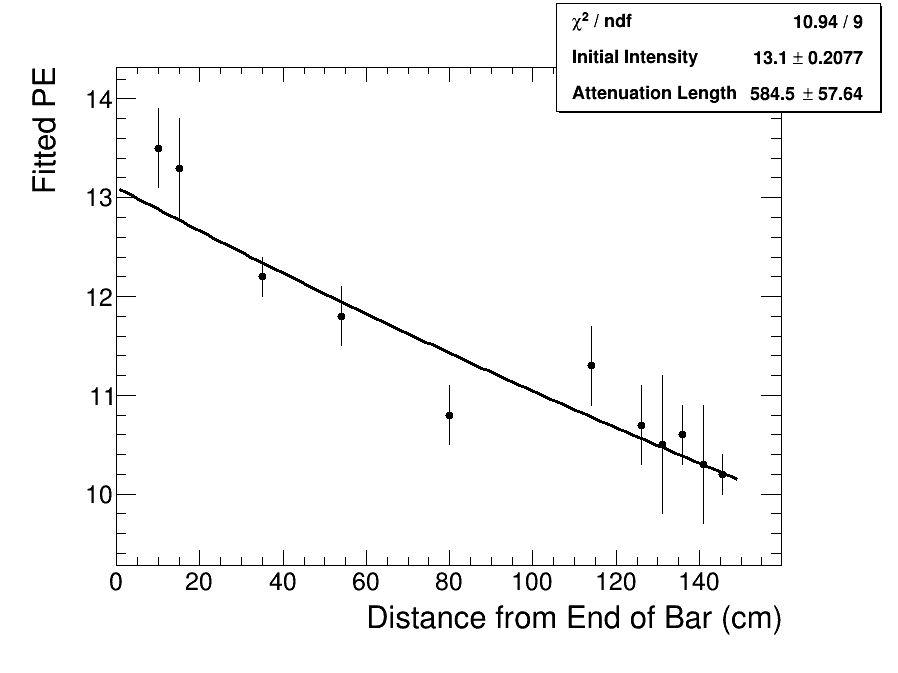
\includegraphics[width=1.0\linewidth]{result_from_attnPlotter.png} 
 \captionof{figure}{The attenuation plot for test stand produced by George Holt. The attenuation length is 580 $\pm$ 60 \hl{units!}} %~can be used as a kind of place holder in latex
 \label{fig:attenuationPlot}
\end{figure}

\section{Modelling Dark Noise}\label{sec:geant4Simulation_ModellingDarkNoise}
Another data driven physical effect modelled in the simulation is the dark noise. Depending on the temperature of the room the electronics in an MPPC will give signals that are non-physical. The dark noise was measured at room temperature by George Holt over a 12 hour period the results in figure \ref{fig:pureDarkNoise} show peaks in units of photo-electrons (PE) with peaks for 1\,PE, 2\,PE and 3\,PE being clearly visible. The MPPC was put inside a container where no light would reach the sensor. 
\begin{figure}[htbp]
 \centering
 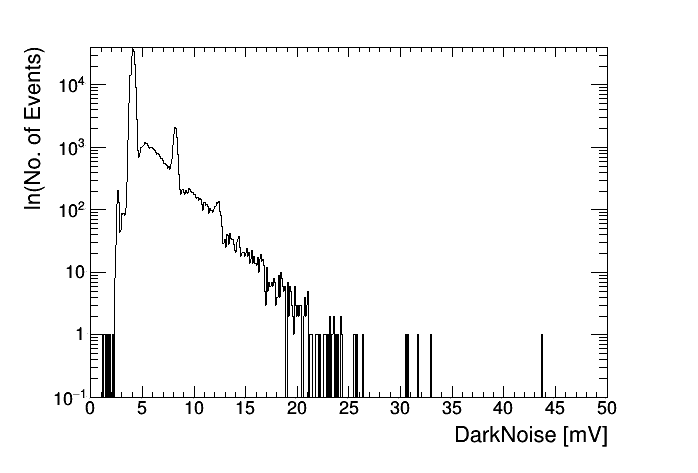
\includegraphics[width=0.8\linewidth]{pureDarkNoise_output.png}
 \captionof{figure}{Dark Noise from the MPPC taken over a period of $\sim$ 12\,hrs. The PE peaks for 1\,PE 2\,PE and 3\,PE can be seen at 4.1\,mv, 8.2\,mv and 12.3\,mv respectively. } %~can be used as a kind of place holder in latex
 \label{fig:pureDarkNoise}
\end{figure}

The dark noise has two distinct components, the peaks and the background surrounding the peaks. The background surrounding the peaks can be modelled using an exponential fit and is done so in figure \ref{subFig:expFitOfDark}. The pedestal peak is also removed and then the exponential is used past 13.7\,mV which can be seen in figure \ref{subFig:fittedDarkNoise}. 
\begin{figure}[htbp]
\centering
\begin{subfigure}{.5\textwidth}
  \centering
  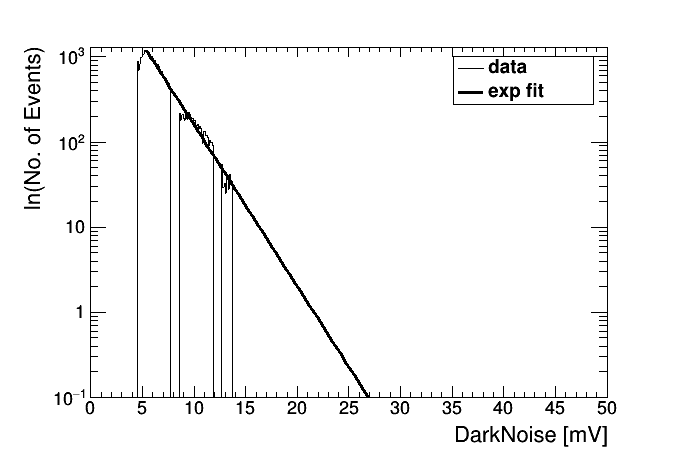
\includegraphics[width=\linewidth]{fit_of_dark_noise.png}
  \captionsetup{width=.9\linewidth}
  \caption{Fit of exponential function using TFit to fit the after-pulsing of the MPPCs}
  \label{subFig:expFitOfDark}
\end{subfigure}%
\begin{subfigure}{.5\textwidth}
  \centering
  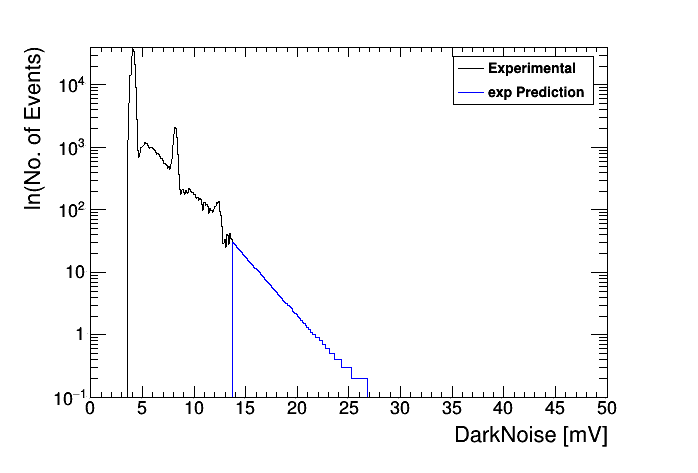
\includegraphics[width=\linewidth]{fittedDarkNoise_output.png}
  \captionsetup{width=.9\linewidth}
  \caption{Fitted exponential past 13.7\,mv once the number of events dropped below 10.}
  \label{subFig:fittedDarkNoise}
\end{subfigure}
\caption{Dark Noise from the MPPC taken over a period of $\sim$ 12\,hrs with an exponential fitted, with a $\chi ^2$ /DOF = 159.748}
\label{fig:fitting_of_non_peak_dark_noise}
\end{figure}

The results from \ref{fig:fitting_of_non_peak_dark_noise} can then be used to construct a cumulative distribution seen in figure \ref{fig:cumulative_prob_dark}, this cumulative distribution is what is used by the simulation in order to visnstruct the dark noise distribution. During the simulation a random dice is thrown that probability is then converted back into a dark noise value which is then assigned to a random bar in the detector. Values past 13.7\,mV use the exponential fit.
\begin{figure}[htbp]
 \centering
 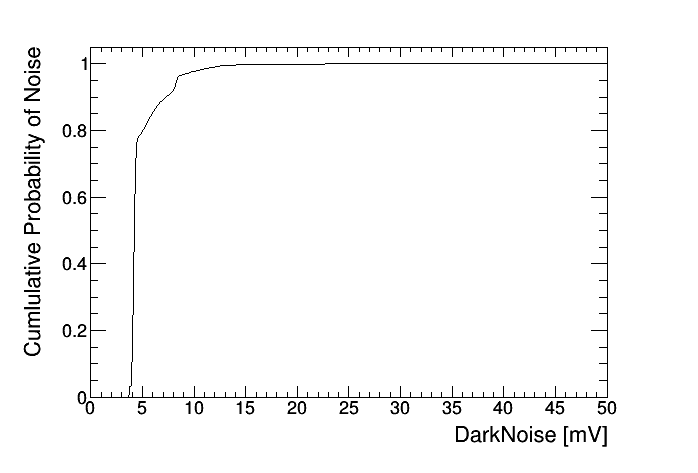
\includegraphics[width=0.8\linewidth]{cumulative_prob_dark_noise.png}
 \captionof{figure}{cumulative probability of the dark noise, which is converted to a table and then searched using the golden section search} %~can be used as a kind of place holder in latex
 \label{fig:cumulative_prob_dark}
\end{figure}
\hl{would be really nice if I could produce a histo of the simulated dark noise and quantify what that looks like and how much we're expecting when we deploy}

\section{Modelling Light Emission}\label{sec:geant4Simulation_ModellingLightEmission}
In order to measure light for a given amount of scintillating material we need to consider several factors. For organic scintillators the type of particle has a significant effect on the absolute light yield. The response of organic scintillators to charged particles can best be described by a relation between $dL/dx$ the fluorescent energy emitted per unit path length and $dE/dx$ the specific energy loss for the charged particle.  A widely used relation first suggested by Birks \cite{birks_1964} is based on the assumption that a high intonation density along the track of the particle leads to quenching from damaged molecules and a lowering of the scintillation efficiency. If we assume that the density of damage molecules along the wake of the particle is directly proportional to the ionisation density we can represent their density by $B(dE/dx)$ where $B$ is a proportionality constant. Birks assumes that some fraction $k$ of theses will lead to quenching\cite{knoll_2010}. A further assumption is that in absence of quenching the light yield is proportional to energy loss shown in equation \ref{equ:light_yield_proportional}. $S$ is the normal scintillation efficiency. To account for the probability of quenching birks then writes equation \ref{equ:Birks_formula}. Equation \ref{equ:Birks_formula} is commonly referred to as Birks formula. As a practical matter the product $kB$ is treated as an adjustable parameter to fit experimental data for a specific scintillator whereas $S$ is particle specific which provides absolute normalisation \cite{knoll_2010}.  
\begin{equation}
\frac{dL}{dx} = S\frac{dE}{dx}
\label{equ:light_yield_proportional}
\end{equation}
\begin{equation}
\frac{dL}{dx} = \frac{S\frac{dE}{dx}}{1 + kB \frac{dE}{dx}}
\label{equ:Birks_formula}
\end{equation}
\\\\In this model molecules in the ionisation column are labelled ``damaged'' and ``undamaged'' for convenience where ``damaged'' molecules are those which dissipate ionisation energy nonradiatively (quenching) and so lower scintillation efficiency\cite{craun_1970} \cite{knoll_2010}. ``Damaged'' molecules occupy highly ionised or excited states, they de-excite quickly ($<$ 1 ns) to the ``undamaged'' condition \cite{craun_1970}. Some permanent damage will occur and does contribute to long term degradation of the scintillator but is not relevant for quenching\cite{craun_1970}. From this B is the ratio of ``damaged''/``undamaged'' molecules and k is the relative probability of quenching. kB is treated as a single adjustable parameter as there is no way to measure k or B separately \cite{craun_1970} \cite{knoll_2010}. Where kB is scintillator dependant only and will be refereed to as a single entity as Birk's constant. The response for electrons above $\sim$ 125\,keV is linear \cite{craun_1970}. This is also seen in Birk's law which also becomes linear for fast electrons \cite{knoll_2010}. This is important for modelling electrons. 
\section{MINERvA Birk's Constant}\label{sec:geant4Simulation_MINERvABirksConstant}
In equation \ref{equ:Birks_formula} the parameters $kB$ and $S$ are empirically determined. $S$ is a normalisation parameter that is particle dependent and kB is the birks constant for the scintillator and is particle independent. The MINERvA collaboration \cite{aliaga_2015} also uses the same scintillator as the VIDARR detector \cite{aliaga_2014}, the collaboration determined the value of the of kB to be 0.0905 $\pm$ 0.015\,mm/MeV at best fit. This Birks parameter was obtained by using GEANT4 MC data, which is the same approach by which VIDARR has obtained its birks parameter.
Both the VIDARR and MINERvA approach use the Geant4 bertini cascade model when attempting to measure the \\\\Birks parameter $kB$ \cite{Heikkinen_2003}. In addition both use the QGSP physics list which applies the quark gluon string model when simulating particles \cite{Patrick_2018}. The steps have to remain course in Geant4 otherwise the $kB$ parameter changes  \cite{aliaga_2015}. This is why the EMY physics lists were not used, even though they simulate smaller steps and so would potentially simulate stopping better. Then energy range for the MINERvA signal is of order $\sim$ 1\,GeV, whereas the energy range for VIDARR's signal is 0-10\,MeV. However a major source of noise for VIDARR are cosmic muons which have energies $\sim$ 1\,GeV and protons with energies between 0-10\,MeV as a result of fast neutrons. Using the minerva data requires going to higher energies (lower $dE/dx$) in order to ensure similar results in the $dL/dx$ fit.  
\\\\The results of the MINERvA Birks law investigation concluded that a birks constant of 0.0905 $\pm$ 0.015\,mm/MeV was the most accurate value for the scintillator \cite{aliaga_2015}. Whilst the MINERvA experiment measures protons with an energy range of 0\,MeV-500\,MeV and the particles of VIDARR's interest are $\overline{\nu_{e}}$s with energy range between 0\,MeV-10\,MeV the Birk's constant is the same regardless. This is because the Birk's law is a representation of the scintillator itself and therefore is not particle or energy dependent, the amount of saturation in the scintillator that the Birks constant represents is constant in all cases. 

\section{Loss of Deposited Energy due to Quenching}\label{sec:geant4Simulation_quenchingLoss}
\hl{Very Important!: This work is currently not replicable, the collection of scripts is on my hepstore somewhere and needs to be backed up and put onto git as soon as possible!}
\\\\The effect of quenching varies greatly depending on the particle it is a function of both energy and mass. By considering three example particles and their corresponding anti-particles the scale of quenching can be observed. The first particle to consider would be electrons as they are one of the most common sources of noise and have a large charge to mass ratio when compared to other particles that could be potential background for this experiment. The level of quenching for electrons and positrons is very minimal which can be seen in figure \ref{fig:electron_positron_quenched_and_not}. This was simulated using a ``slab'' of material, figure \ref{fig:electrons_viewed_in_slab}, instead of using a bar or a full detector this was done to ensure that all of the energy was kept inside the plastic scintillator so that the full energy loss due to quenching could be measured. 

\begin{figure}[htbp]
\centering
\begin{subfigure}{.5\textwidth}
  \centering
  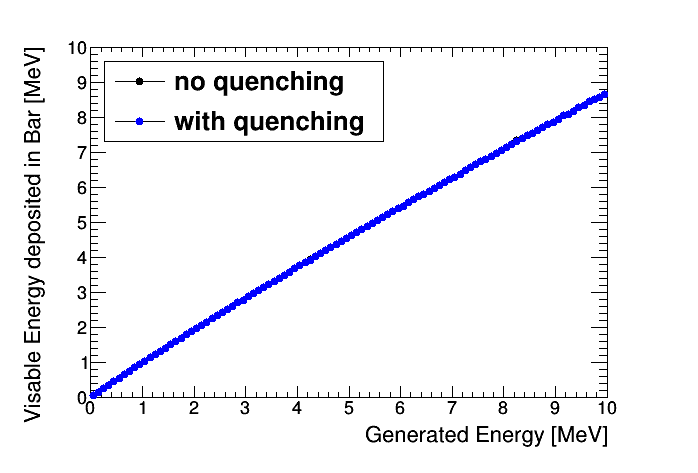
\includegraphics[width=\linewidth]{quench_eng_LinElectrons.png}
  \captionsetup{width=.9\linewidth}
  \caption{Visible electron energy deposition with and without quenching}
  \label{subFig:electron_quenched_and_not}
\end{subfigure}%
\begin{subfigure}{.5\textwidth}
  \centering
  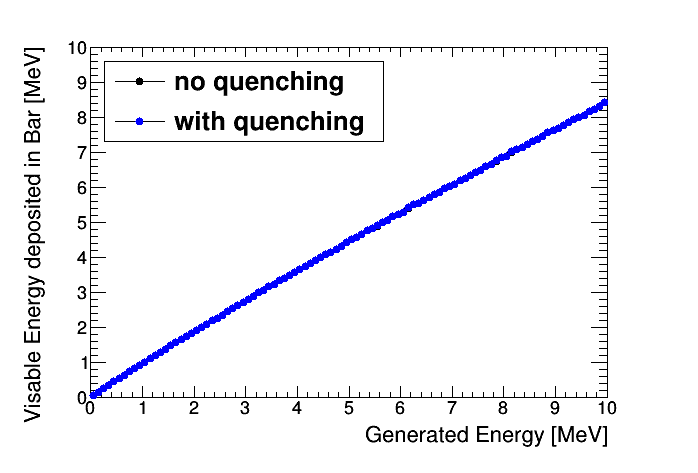
\includegraphics[width=\linewidth]{quench_eng_LinPositrons.png}
  \captionsetup{width=.9\linewidth}
  \caption{Visible positron energy deposition with and without quenching}
  \label{subFig:positron_quenched_and_not}
\end{subfigure}
\caption{Electrons and positrons visible energy with and without quenching in a ``slab'' of material}
\label{fig:electron_positron_quenched_and_not}
\end{figure}

\begin{figure}[htbp]
\centering
\begin{subfigure}{.5\textwidth}
  \centering
  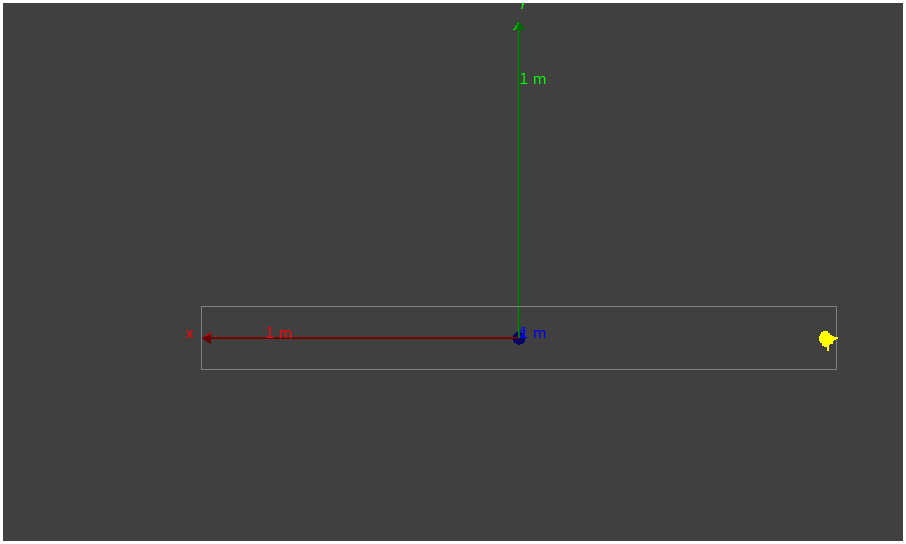
\includegraphics[width=\linewidth]{e-_10MeV_Length_on_view.png}
  \captionsetup{width=.9\linewidth}
  \caption{electrons side on view in ``slab''}
  \label{subFig:electron_side_slab}
\end{subfigure}%
\begin{subfigure}{.5\textwidth}
  \centering
  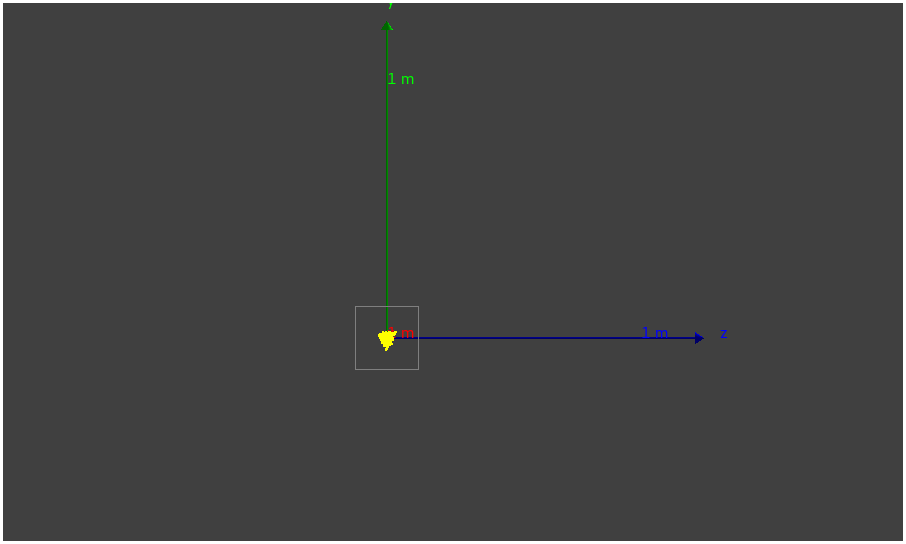
\includegraphics[width=\linewidth]{e-_10MeV_side_on_view.png}
  \captionsetup{width=.9\linewidth}
  \caption{electron length on view in ``slab''}
  \label{subFig:electron_length_slab}
\end{subfigure}
\caption{Electron side and length on view in ``slab'' of material, the electrons are not leaving the material.}
\label{fig:electrons_viewed_in_slab}
\end{figure}

The effect of quenching on protons is much more significant than for electrons, this is because the charge for protons is equal and opposite for electrons but the mass is $\sim$ 2000 times greater than for electrons. This results in a large amount of energy no longer being deposited in the scintillator which can be seen in figure \ref{fig:proton_Apronton_quenched_and_not} which shows both the energy deposition of protons and anti-protons. In figures \ref{subFig:proton_quenched_and_not}, \ref{subFig:Aproton_quenched_and_not} the energy deposition is linear for protons and anti-protons without quenching this suggests that the majority of the energy lost is lost via quenching. For $\alpha$ particles the effect is even more significant $\alpha$ particles which are 4 times more massive than protons but have twice the charge. The effect of quenching is $\sim$ 4 times greater for $\alpha$ particles than for protons which can be seen when comparing the energy deposited in the slab for figures \ref{fig:proton_Apronton_quenched_and_not} and \ref{fig:alpha_Aalpha_quenched_and_not}. 

\begin{figure}[htbp]
\centering
\begin{subfigure}{.5\textwidth}
  \centering
  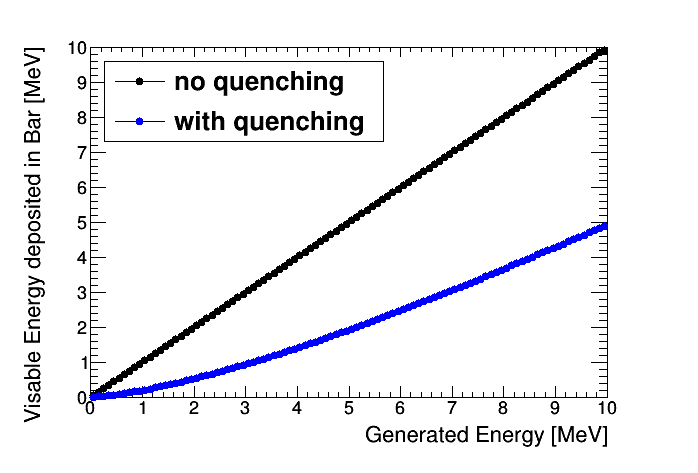
\includegraphics[width=\linewidth]{quench_eng_protons.png}
  \captionsetup{width=.9\linewidth}
  \caption{Visible proton energy deposition with and without quenching}
  \label{subFig:proton_quenched_and_not}
\end{subfigure}%
\begin{subfigure}{.5\textwidth}
  \centering
  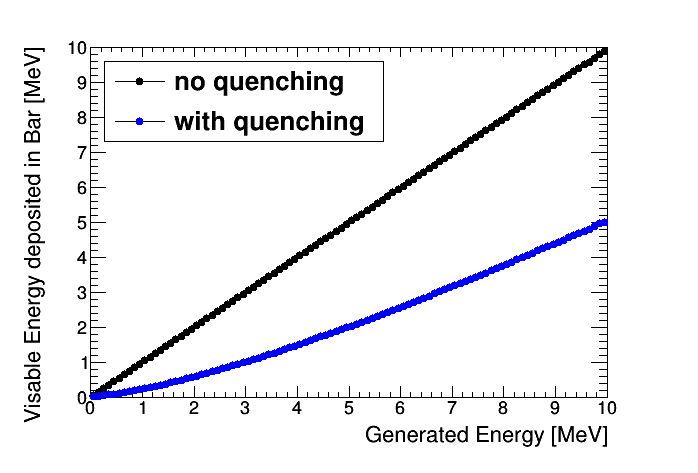
\includegraphics[width=\linewidth]{quench_eng_Aprotons.png}
  \captionsetup{width=.9\linewidth}
  \caption{Visible anti-proton energy deposition with and without quenching}
  \label{subFig:Aproton_quenched_and_not}
\end{subfigure}
\caption{protons and anti-protons visible energy with and without quenching in a ``slab'' of material}
\label{fig:proton_Apronton_quenched_and_not}
\end{figure}

\begin{figure}[htbp]
\centering
\begin{subfigure}{.5\textwidth}
  \centering
  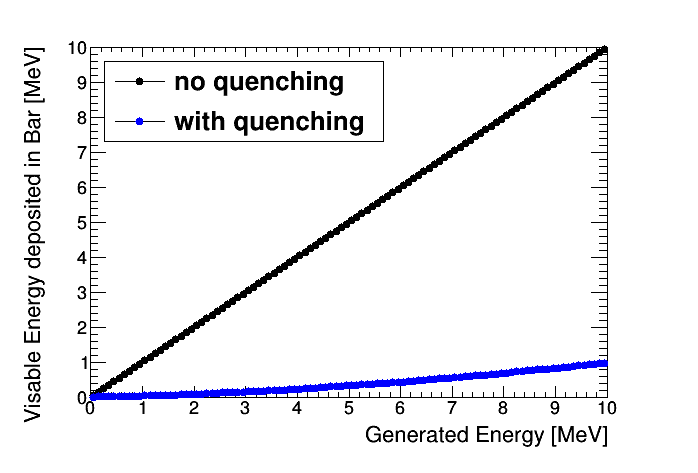
\includegraphics[width=\linewidth]{quench_eng_Alpha.png}
  \captionsetup{width=.9\linewidth}
  \caption{Visible alpha particle energy deposition with and without quenching}
  \label{subFig:alpha_quenched_and_not}
\end{subfigure}%
\begin{subfigure}{.5\textwidth}
  \centering
  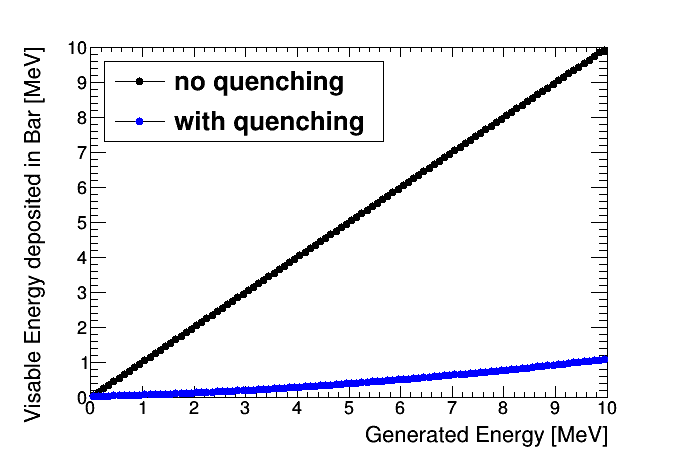
\includegraphics[width=\linewidth]{quench_eng_AAlpha.png}
  \captionsetup{width=.9\linewidth}
  \caption{Visible anti-alpha particle energy deposition with and without quenching}
  \label{subFig:Aalpha_quenched_and_not}
\end{subfigure}
\caption{alpha and anti-alpha particles visible energy with and without quenching in a ``slab'' of material}
\label{fig:alpha_Aalpha_quenched_and_not}
\end{figure}

\section{Monte Carlo Modelling of Birks Law}\label{sec:geant4Simulation_MonteCarloBirksLaw}
\hl{Very Important!: This work is currently not replicable, the collection of scripts is on my hepstore somewhere and needs to be backed up and put onto git as soon as possible!}
\\\\The photon model in Geant4 is computationally expensive as the simulation toolkit simulates optical photon tracks at every energy deposition for a given amount of energy. With a scintillation yield of $10^5$\,ph/MeV as in this simulation the slowdown observed at higher energies is extreme. This slowdown can be somewhat alleviated by counting the number of photons and then killing the optical photon tracks, as it is the number of photons produced that determines quenching, but even this is still computationally expensive. So whilst the count and kill method was used for determining Birk's law, once the light was characterised the count and kill method was abandoned due to its high computational load.
\\\\In order to accurately quantify the response of Birks law Monte Carlo modelling was used in Geant4. This was done so that the value of $S$ in equation \ref{equ:Birks_formula} could be found for each particle. The Geant4 physics list of QGSP\_\_BERT\_\_HP allows for good repdouction of Birk's law \cite{Patrick_2018},\cite{aliaga_2015}. However, two new models of the scintillator were required in order to accurately quantify the effects of the Birk's constant, both of them required the removal of all wavelength shifting fibres and MPPCs and so are just scintillator. The first model was a ``slice model'' that was 1\,mm thick and had a cross section of 0.2\,m by 0.2\,m, this allowed for the approximations $dL/dx \approx \Delta L / \Delta x$ and $dE/dx \approx \Delta E / \Delta x$ to be used. The second model was a ``slab'' model (figure \ref{fig:electrons_viewed_in_slab}) that was 2\,m thick and had a cross section of 0.2\,m by 0.2\,m, this model was used for determining how effective the Birk's approximation was. Both models had particle energy ranges of 0\,MeV-100\,MeV.
The ``slice'' model was used to determine the $S$ values for every particle in equation \ref{equ:Birks_formula}, once those had been obtained the $kB$ value of 0.0905 $\pm$ 0.015\,mm/MeV obtained from MINERvA was also used. By using the approximations $dL/dx \approx \Delta L / \Delta x$ and $dE/dx \approx \Delta E / \Delta x$ and using $\Delta L = L_{\textrm{end}} - L_{\textrm{start}} $ where in the simulation it is known the light at the start of the step $L_{\textrm{start}} = 0$ and $L_{\textrm{end}}$ is the Light at the end of each Geant4 step allows for equation \ref{equ:light_produced} to be created. Using equation \ref{equ:light_produced} the light yeild can now be calculated, the following particles were simulated: $e^-$,$e^+$,$p$,$\overline{p}$,$\pi^+$,$\pi^-$,$\mu^-$,$\mu^+$,$\alpha$,$\overline{\alpha}$. 
\begin{equation}
L_{\textrm{end}}\approx \Delta x \left(\frac{S\frac{\Delta E}{\Delta x}}{1 + kB \frac{\Delta E}{\Delta x}}\right) 
\label{equ:light_produced}
\end{equation}
The approximations that the Birks law predicts for $p$,$\overline{p}$,$\pi^+$,$\pi^-$,$\mu^-$,$\mu^+$,$\alpha$,$\overline{\alpha}$ are very close to the model of light that Geant4 predicts. The deviation from Geant4 is at the worst at 100\,MeV where there is a deviation of $\sim$ $3\%$ in light output between Geant4 and the Birks approximation of protons and anti-protons seen in figure \ref{fig:proton_aproton_light} with \ref{subFig:proton_light} representing protons and \ref{subFig:aproton_light} representing anti-protons. The Brik's approximation proves to be a closer fit to the data than the simulated light fit which is a square function ($L = aE^2 + bE+ c$). \hl{IMPORTANT NOTE TO SELF: The chisq/ndf are awful in both cases, but there must be a way to show one is better than the other.}
\begin{figure}[htbp]
\centering
\begin{subfigure}{.5\textwidth}
  \centering
  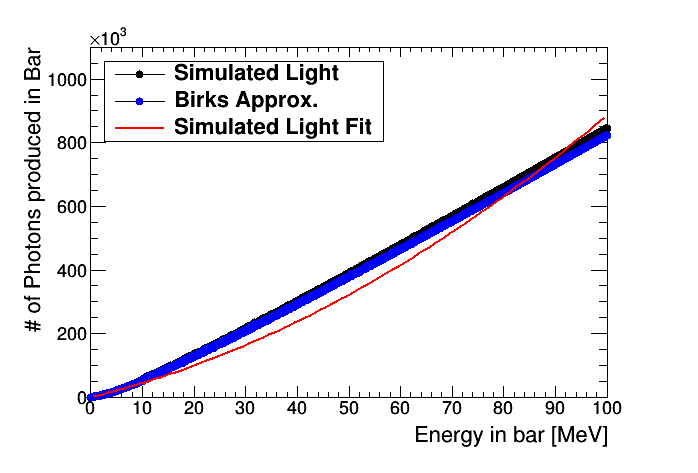
\includegraphics[width=\linewidth]{light_of_protons0-100mev.png}
  \captionsetup{width=.9\linewidth}
  \caption{proton light produced by Geant4 compared to the Birks approximation of that light, the simulated light fit is the square funciton $L = aE^2 + bE+ c$ and is fit to the Geant4 simulated light}
  \label{subFig:proton_light}
\end{subfigure}%
\begin{subfigure}{.5\textwidth}
  \centering
  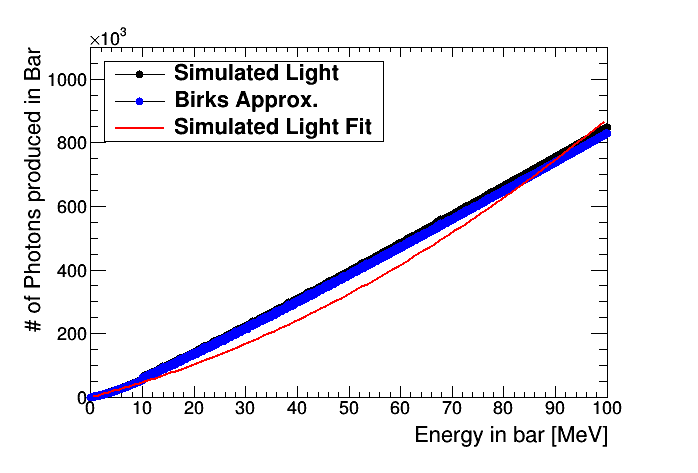
\includegraphics[width=\linewidth]{light_of_Aprotons0-100mev.png}
  \captionsetup{width=.9\linewidth}
  \caption{anti-proton light produced by Geant4 compared to the Birks approximation of that light, the simulated light fit is the square funciton $L = aE^2 + bE+ c$ and is fit to the Geant4 simulated light}
  \label{subFig:aproton_light}
\end{subfigure}
\caption{proton and anti-proton light output compared to the birks approximation and a square fit to the light out put in Geant4}
\label{fig:proton_aproton_light}
\end{figure}
However the light yield for electrons and positrons seen in figure \ref{fig:electron_positron_light} varies more significantly. A variation of $\sim$ 15\,\% is seen in the electrons, figure \ref{subFig:electron_light}, and a variation and a variation of $\sim$ 20\,\% is seen in positrons, figure \ref{subFig:positron_light} at maximum energy values. In figure \ref{fig:electron_positron_light}, the simulated light fit, which is a square fit to the data in the form $L = aE^2 + bE+ c$ fits the data far closer. Figure \ref{fig:square_electron_positron_light} shows this approximation inputted instead, there is a slight variation between the simulated light fit and the square approx. seen in figures \ref{subFig:square_electron_light} and \ref{subFig:square_positron_light}. This is because the simulated light fit is fitted to the whole light distribution whereas the light of the square approximation is produced per Geant4 step. Despite this, the square approximation of light for electrons ($L = 0.9347E^2 + 10340E - 0.1000$) had a variation of 0.7\,\% at maximum energy and the square approximation of the light for the positrons ($L = 0.9716E^2 + 10350E -0.1000$) had a variation of 0.3\,\% at maximum energy. 
\begin{figure}[htbp]
\centering
\begin{subfigure}{.5\textwidth}
  \centering
  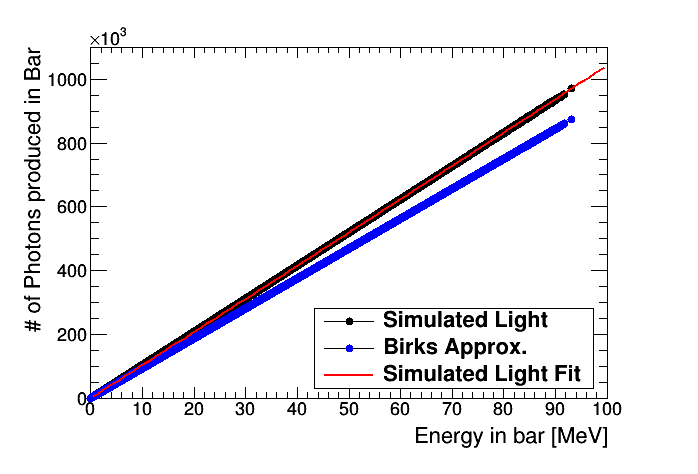
\includegraphics[width=\linewidth]{light_of_electrons0-100mev.png}
  \captionsetup{width=.9\linewidth}
  \caption{Electron light produced by Geant4 compared to the Birks approximation of that light, the simulated light fit is the square funciton $L = aE^2 + bE+ c$ and is fit to the Geant4 simulated light}
  \label{subFig:electron_light}
\end{subfigure}%
\begin{subfigure}{.5\textwidth}
  \centering
  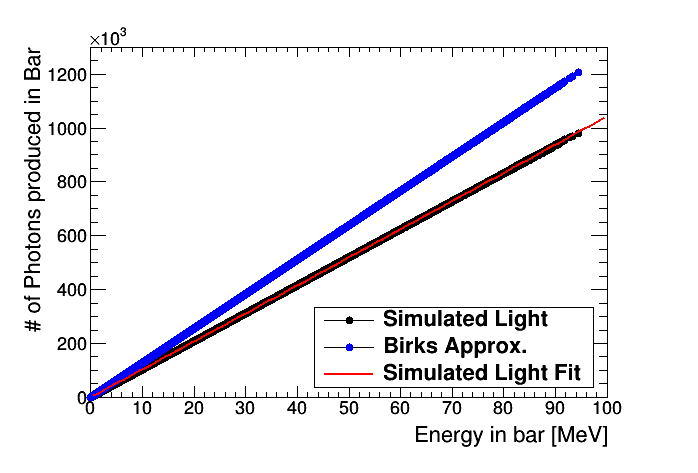
\includegraphics[width=\linewidth]{light_of_positrons0-100mev.png}
  \captionsetup{width=.9\linewidth}
  \caption{Positron light produced by Geant4 compared to the Birks approximation of that light, the simulated light fit is the square funciton $L = aE^2 + bE+ c$ and is fit to the Geant4 simulated light}
  \label{subFig:positron_light}
\end{subfigure}
\caption{Electron, Positron light output compared to the birks approximation and a square fit to the light out put in Geant4}
\label{fig:electron_positron_light}
\end{figure}
\begin{figure}[htbp]
\centering
\begin{subfigure}{.5\textwidth}
  \centering
  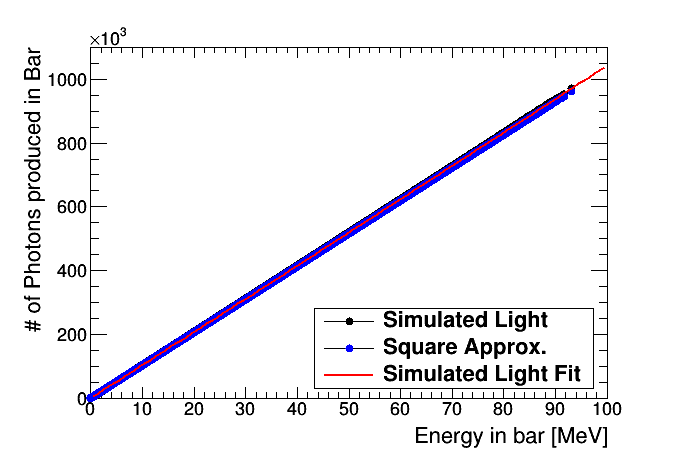
\includegraphics[width=\linewidth]{light_of_electronsLin0-100mev.png}
  \captionsetup{width=.9\linewidth}
  \caption{Electron light simulated by Geant4 compared to the square approximation $L = aE^2 + bE+ c$ }
  \label{subFig:square_electron_light}
\end{subfigure}%
\begin{subfigure}{.5\textwidth}
  \centering
  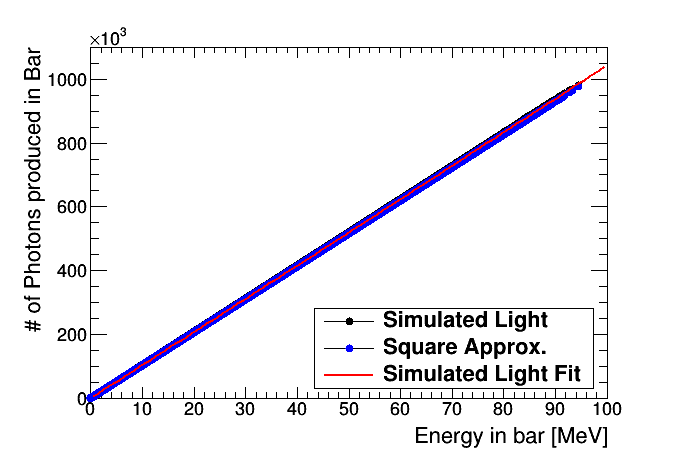
\includegraphics[width=\linewidth]{light_of_positronsLin0-100mev.png}
  \captionsetup{width=.9\linewidth}
  \caption{Positron light simulated by Geant4 compared to the square approximation $L = aE^2 + bE+ c$}
  \label{subFig:square_positron_light}
\end{subfigure}
\caption{Electron and positron light output from simulation compared to a Geant4 step square approximation}
\label{fig:square_electron_positron_light}
\end{figure}
The conversion for light into energy for electrons in figure \ref{subFig:square_electron_light} is defined by equation \ref{equ:MeV_electron_equivalent_square}. The light of an electron is the highest amount of light per MeV that a particle can deposit this MeV electron equivalent (MeVee) is a special nomenclature used to describe the absolute light yeild \cite{knoll_2010}. As the squared term $ << $ the linear term, the squared term is ignored for the purposes of light conversion, producing equation \ref{equ:MeV_electron_equivalent_linear}. By rearranging equation \ref{equ:MeV_electron_equivalent_linear} for energy production we then get equation \ref{equ:MeV_electron_equivalent_light} which allows for the conversion from the Birks approximation of light into the energy or the square approximation of light into energy for the electrons and positrons. With equation \ref{equ:MeV_electron_equivalent_light} it is possible to show the energy loss due to quenching, once the L in equation \ref{equ:MeV_electron_equivalent_light} is substituted with the light at the end of the Geant4 step shown in equation \ref{equ:light_produced}. \hl{IMPORTANT NOTE TO SELF: Again chisqs for this are very very poor, but I don't know how to make better, must return to this at a later date!} 
\begin{equation}
L = 0.9347E^2 + 10340E - 0.1000
\label{equ:MeV_electron_equivalent_square}
\end{equation}
\begin{equation}
L = 10340E - 0.1000
\label{equ:MeV_electron_equivalent_linear}
\end{equation}
\begin{equation}
E = \frac{L +0.1000}{10340} 
\label{equ:MeV_electron_equivalent_light}
\end{equation}

\section{Counting Statistics} \label{sec:geant4Simulation_countingStats}
When a particle passes through the scintillating plastic it produces photons as it interacts. These photons then travel through the bar until they meet the wavelength shifting fibres (wls). The photons then travel down the wls until they encounter the MPPC  this signal is them amplified by the MPPC producing a signal of 4.2\,mV which is equivalent for one photon see figure \ref{fig:pureDarkNoise} which is called a photo-electron equivalent (PE). So for n number of photo-electron equivalents there will be a Poisson distribution (equation \ref{equ:possionProb}) associated with it due to counting statistics. This only holds true if there is a small probability of a given outcome which is true for this case. For this distribution $pn = \overline{x}$ where $\overline{x}$ is the expectation value, substituting this into equation \ref{equ:possionProb} we get equation \ref{equ:possionExpectation} \cite{knoll_2010}.
\begin{equation}
P(x) = \frac{(pn)^x e^{-pn}}{x!}  
\label{equ:possionProb}
\end{equation}

\begin{equation}
P(x) = \frac{(\overline{x})^x e^{-\overline{x}}}{x!}  
\label{equ:possionExpectation}
\end{equation}

Further the variance of this model can thus be explained using equation  \ref{equ:possionVar} which also gives $\sigma^2 = \overline{x}$ and thus gives a standard deviation of $\sigma = \sqrt{\overline{x}}$ \cite{knoll_2010}. This definition is also of the standard deviation is also true for the Gaussian distribution. The Gaussian distribution which uses this standard deviation can be seen in equation \ref{equ:guassianExpectation}. When n is high enough the Poisson distribution will approximate to a Gaussian distribution this is useful when simulating light counting statistics because a Gaussian distribution is much less computationally intensive as there is no factorial. The point where Gaussian is used instead of Poisson in the simulation is at a value of 10 photons seen in figure \ref{fig:CoutingStats10}, this is when 99.9\,\% of the distribution having 2 photons which is the limit for hits to be considered. 

\begin{equation}
\sigma ^2 \equiv \sum_{x=0}^{n} (x-\overline{x})^2 P(x) = pn = \overline{x} 
\label{equ:possionVar}
\end{equation}

\begin{equation}
P(x) = \frac{1}{\sigma \sqrt[]{2 \pi}} \exp \left(-\frac{1}{2}\left(\frac{x-\overline{x}}{\sigma}\right)^{2}\right)
\label{equ:guassianExpectation}
\end{equation}

\begin{figure}[htbp]
 \centering
 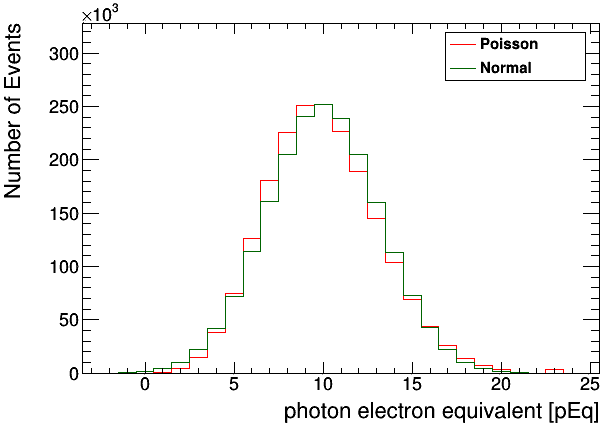
\includegraphics[width=0.8\linewidth]{countingStats10.png}
 \captionof{figure}{Counting statistics for poission and normal distribution for an expectation value of 10 photons the normal distribution is used past when the expectation value is 10 photons or higher to save on computational load.} %~can be used as a kind of place holder in latex
 \label{fig:CoutingStats10}
\end{figure}

\section{Simulated Results With Physical and Electronic Effects}\label{sec:geant4Simulation_resultsPhysicalElectronics}
The impact of physical and electronic effects on simulated data is quite significant especially for heavier particles such as protons and $\alpha$s. The heaviest particle we expect to see in statistically significant quantities is the $\alpha$ in order to show the maximum difference between generated and more realistic simulation generated $\alpha$ particles are used for this section. 
\\\\If these effects are left out of the simulation then the results look nonphysical in figure \ref{fig:alpha_summed_vs_truth} the summed energy inside the detector is equal to the truth energy in most cases. The only events which do not have all the energy summed in the detector are those which were generated near the edges of the bar, these events are absorbed by the TiO$_2$ coating and so deposit less energy in the detector. The modelling of quenching (see section \ref{sec:geant4Simulation_MonteCarloBirksLaw}) and attenuation (see figure \ref{fig:attenuationPlot}) therefore cause a large decrease in the summed energy inside the detector seen in figure \ref{fig:alphaVisVsTruthZoom}. This version of the data can be seen as what an idealistic version of the VIDARR detector could produce. The detector response is longer linear due to he effects described by Birk's Law. 
\begin{figure}[htbp]
 \centering
 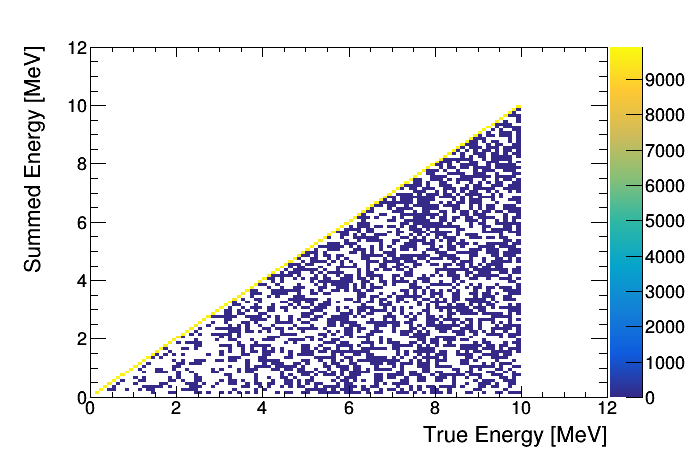
\includegraphics[width=0.7\linewidth]{truth_vs_summed_alpha.png}
 \captionof{figure}{The energy deposited in a simulated detector by $\alpha$ particles without physical and electronic effects taken into account, this is the maximum possible energy that can be deposited.} %~can be used as a kind of place holder in latex
 \label{fig:alpha_summed_vs_truth}
\end{figure}
\begin{figure}[htbp]
 \centering
 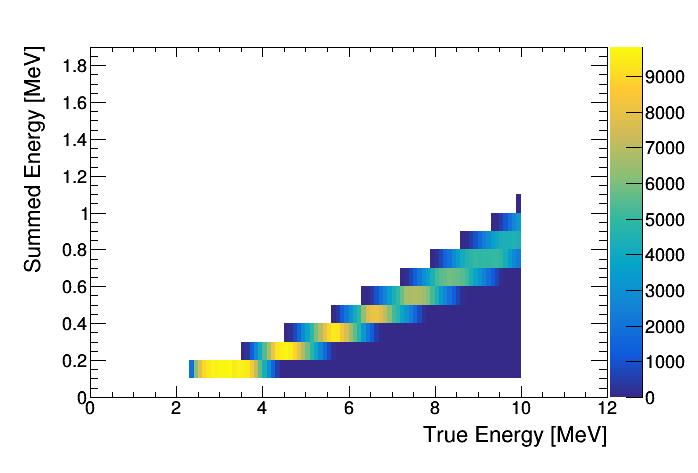
\includegraphics[width=0.7\linewidth]{Chapter4/Figs/Raster/truth_vs_visSummed_alpha_zoom.png}
 \captionof{figure}{The energy deposited in a simulated detector by $\alpha$ particles with only the physical effects of quenching and attenuation taken into account. The detector effects of dark noise and counting statistics are not taken into account} %~can be used as a kind of place holder in latex
 \label{fig:alphaVisVsTruthZoom}
\end{figure}


Finally the effects caused by the electronics and the counting statistics (figure \ref{fig:CoutingStats10}) gives the simulated distribution a more realistic shape. The results for this can be seen in figure \ref{fig:alphaRecoVsTruthZoom}. With the data driven effects taken into account the simulation should give a more realistic result. Unfortunately due to the outbreak of Covid-19 the detector construction was delayed and so the accuracy of this simulation can only be benched marked against the individual components rather than the detector as a whole. 
\begin{figure}[htbp]
 \centering
 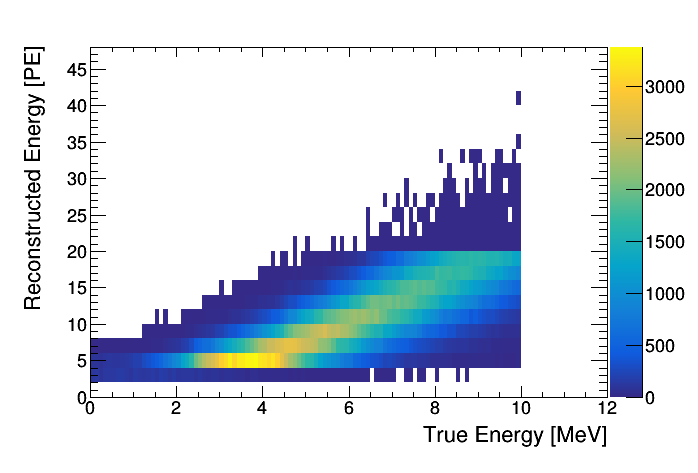
\includegraphics[width=0.7\linewidth]{Chapter4/Figs/Raster/truth_vs_recoSummed_alpha_zoom.png}
 \captionof{figure}{The energy deposited in a simulated detector by $\alpha$ particles with physical effects of quenching and attenuation taken into account as well as the detector effects of dark noise and counting statistics.} %~can be used as a kind of place holder in latex
 \label{fig:alphaRecoVsTruthZoom}
\end{figure}

\section{Modelling Gadolinium}\label{sec:geant4Simulation_modellingGadolinium}
Gadolinium is useful for measuring inverse $\beta$ decay as when the neutron is given off and subsequently absorbed by the layer of gadolinium in between the layers of scintillating plastic in the VIDARR detector a delayed 8\,MeV $\gamma$ cascade is released. This is the trigger signal for the VIDARR detector. After the cascade has been triggered on the detector looks backwards in time to determine the positron cluster. 
\\\\Gadolinium has two models in Geant 4 the photon evaporation model seen in \ref{subFig:differentGeant4Models_photonEvaporationGd} and the final state model seen in  \ref{subFig:differentGeant4Models_finalStateGd}. These two models have different strengths and weaknesses the photon evaporation model conserves energy by ``boiling off'' the known decay energies of Gadolinium until there is no more energy left to disperse. This approach attempts to match the multiplicity of the gadolinium cascade but in so doing the high energy $\gamma$ rays that are the most indicative of the gadolinium cascade are not present. The other model in Geant 4 is the final state model which tries to match the spectrum of measured energy rays. However, by using this approach the conservation of energy is violated. Of the two models the final state would be preferred in the case of inverse $\beta$ decay because the high energy $\gamma$ rays are used to distinguish the gadolinium cascade from background.

\begin{figure}[htbp]
\centering
\begin{subfigure}{.5\textwidth}
  \centering
  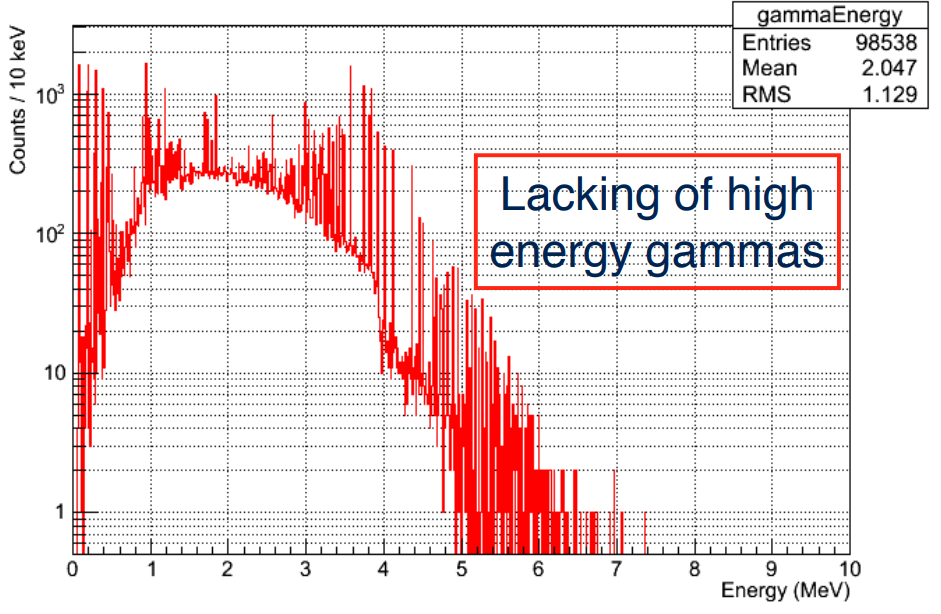
\includegraphics[width=\linewidth]{Chapter4/Figs/Raster/gadolinium/photonEvaporationGd.png}
  \captionsetup{width=.9\linewidth}
  \caption{Energies of single $\gamma$ rays from the photon evaporation model in Geant 4 this conserves energy but does not have high energy $\gamma$ rays that are typically associated with natural gadolinium. From \cite{YuChen_2015}. }
  \label{subFig:differentGeant4Models_photonEvaporationGd}
\end{subfigure}%
\begin{subfigure}{.5\textwidth}
  \centering
  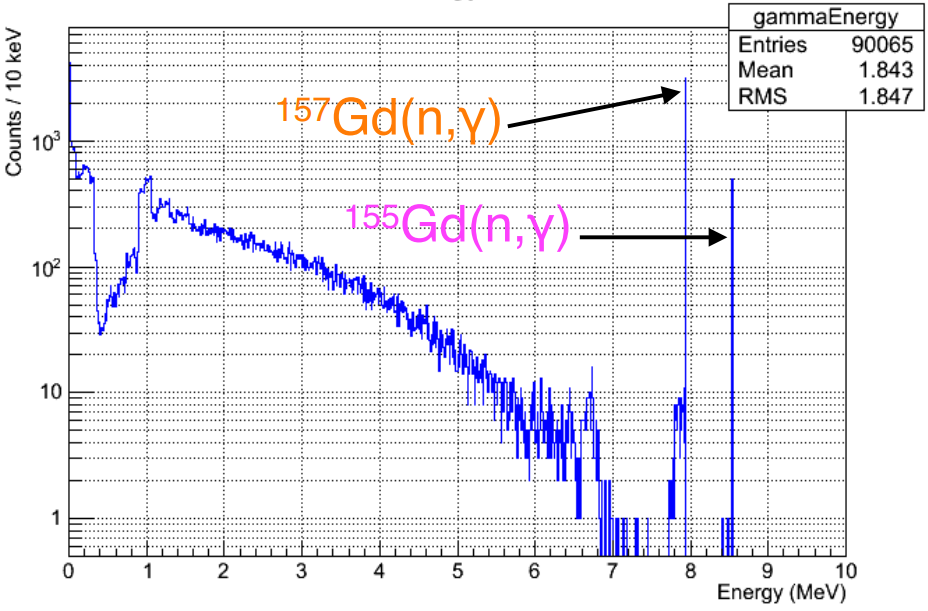
\includegraphics[width=\linewidth]{Chapter4/Figs/Raster/gadolinium/FinalStateGd.png}
  \captionsetup{width=.9\linewidth}
  \caption{Energies of the $\gamma$ rays from the final state model in Geant 4 this shows the high energy gamma rays from both $^{157}$Gd and $^{155}$Gd however this does break the conservation of energy. From \cite{YuChen_2015}. }
  \label{subFig:differentGeant4Models_finalStateGd}
\end{subfigure}
\caption{The energies of $\gamma$ rays of both the photon evaporation model and the final state model.}
\label{fig:differentGeant4Models}
\end{figure}

% \begin{figure}[htbp]
%  \centering
%  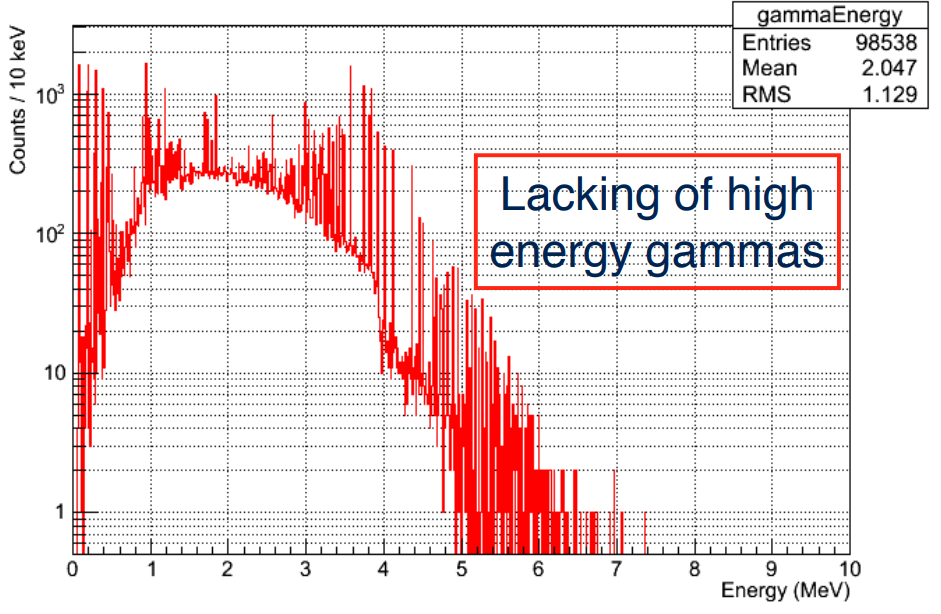
\includegraphics[width=0.7\linewidth]{Chapter4/Figs/Raster/gadolinium/photonEvaporationGd.png}
%  \captionof{figure}{blah.} %~can be used as a kind of place holder in latex
%  \label{fig:photonEvaporationGd}
% \end{figure}

% \begin{figure}[htbp]
%  \centering
%  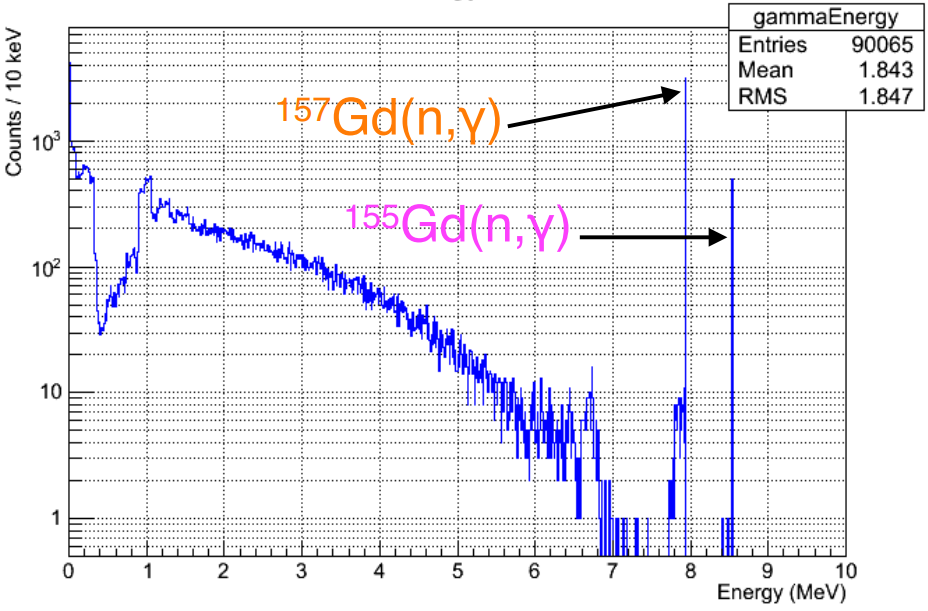
\includegraphics[width=0.7\linewidth]{Chapter4/Figs/Raster/gadolinium/FinalStateGd.png}
%  \captionof{figure}{blah.} %~can be used as a kind of place holder in latex
%  \label{fig:FinalStateGd}
% \end{figure}

\begin{figure}[htbp]
 \centering
 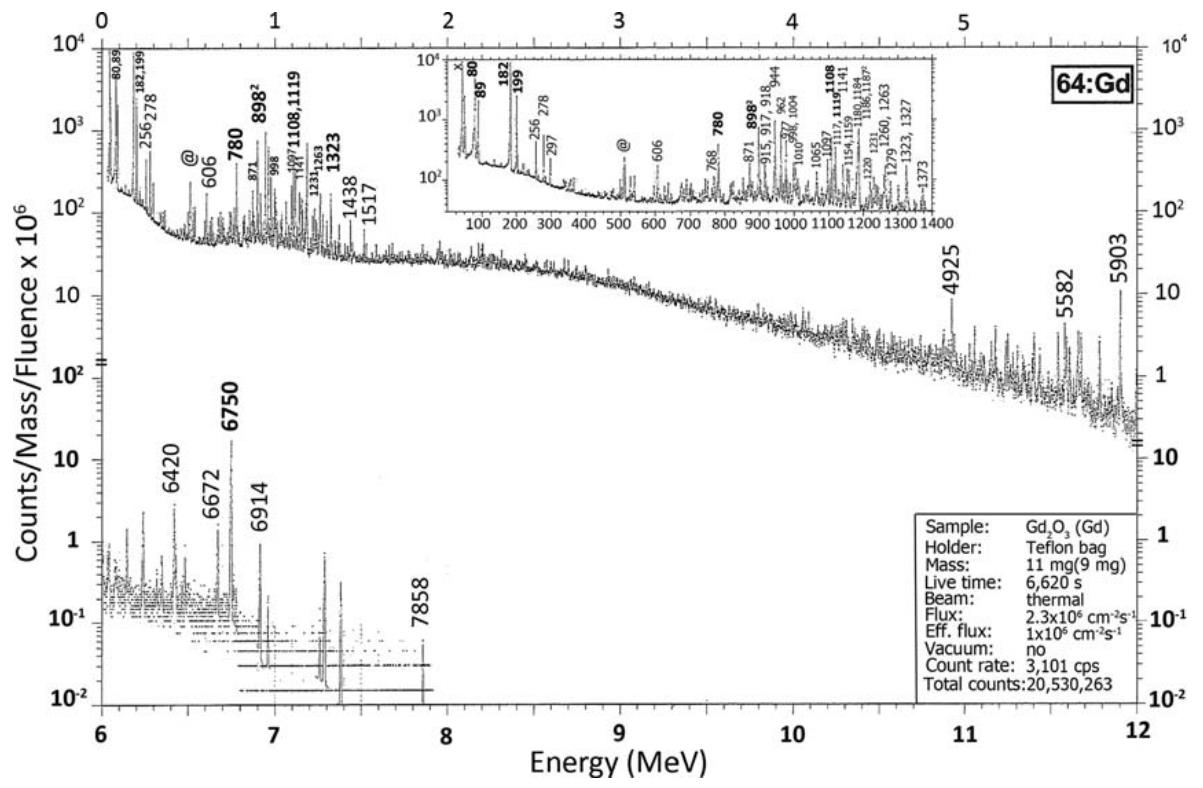
\includegraphics[width=0.7\linewidth]{Chapter4/Figs/Raster/gadolinium/naturalGd.png}
 \captionof{figure}{Natural Gadolinium gamma spectra from \cite{molnar_2004}} %~can be used as a kind of place holder in latex
 \label{fig:naturalGd.png}
\end{figure}

\begin{figure}[htbp]
 \centering
 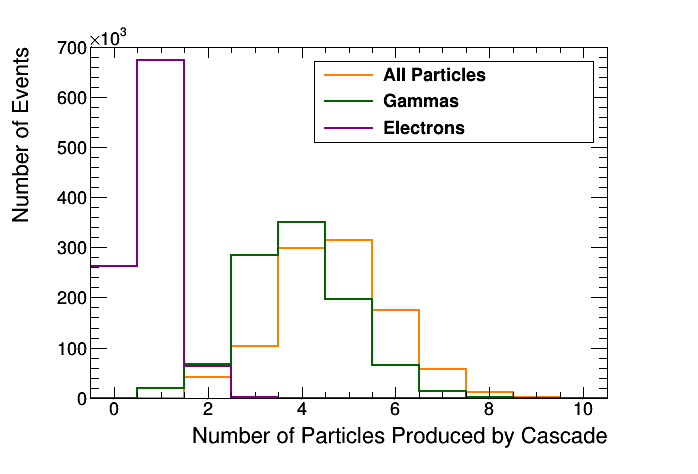
\includegraphics[width=0.7\linewidth]{Chapter4/Figs/Raster/gadolinium/gadoliniumMultipliciesBreakdownCascade.png}
 \captionof{figure}{Multiplicities from the DANCE dicebox based on the DANCE experimental data for $^{157}$Gd \cite{Chyzh_2011}. } %~can be used as a kind of place holder in latex
 \label{fig:gadoliniumMultipliciesBreakdownCascade}
\end{figure}

\begin{figure}[htbp]
 \centering
 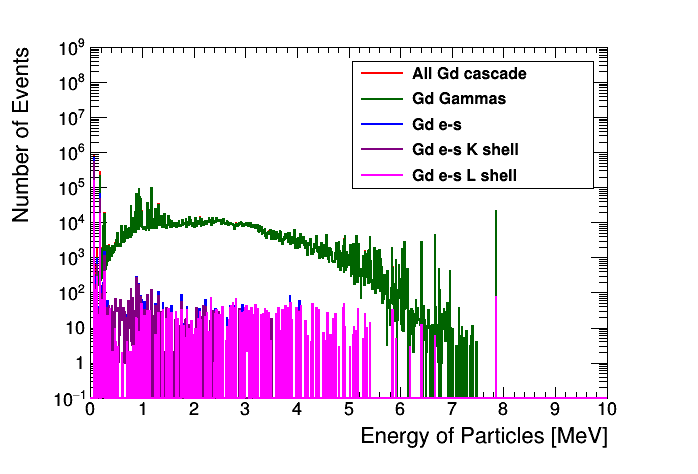
\includegraphics[width=0.7\linewidth]{Chapter4/Figs/Raster/gadolinium/gadoliniumEnergiesCascade.png}
 \captionof{figure}{Energies from the DANCE dicebox based on the DANCE experimental data for $^{157}$Gd \cite{Chyzh_2011}. } %~can be used as a kind of place holder in latex
 \label{fig:gadoliniumEnergiesCascade}
\end{figure}

% \begin{figure}[htbp]
%  \centering
%  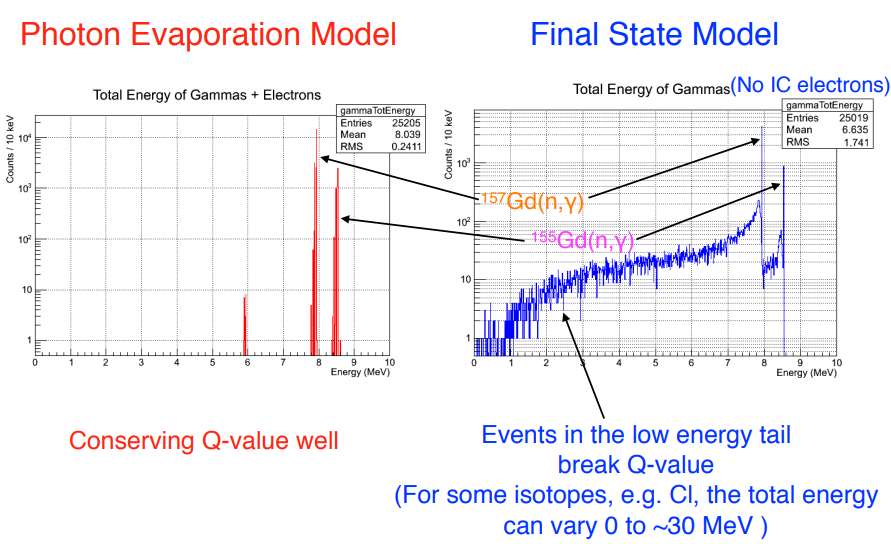
\includegraphics[width=0.7\linewidth]{Chapter4/Figs/Raster/gadolinium/pe_vs_fs_models_summed.png}
%  \captionof{figure}{blah.} %~can be used as a kind of place holder in latex
%  \label{fig:pe_vs_fs_models_summed}
% \end{figure}

\begin{figure}[htbp]
 \centering
 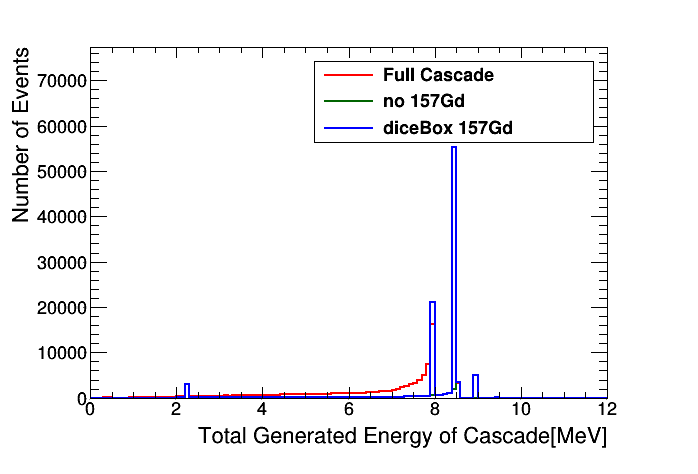
\includegraphics[width=0.7\linewidth]{Chapter4/Figs/Raster/gadolinium/TotalGeneratedEnergyOfCascadeFinalStateDicebox.png}
 \captionof{figure}{Total generated energy of the cascade the dicebox based on the DANCE detector data \cite{Chyzh_2011}.} %~can be used as a kind of place holder in latex
 \label{fig:TotalGeneratedEnergyOfCascadeFinalStateDicebox}
\end{figure}

\begin{figure}[htbp]
 \centering
 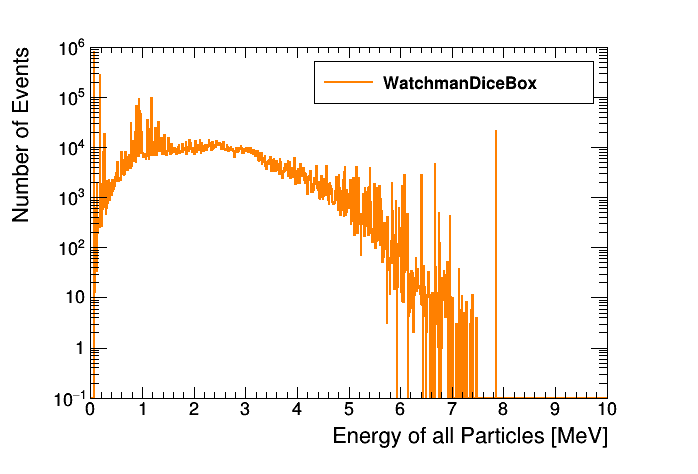
\includegraphics[width=0.7\linewidth]{Chapter4/Figs/Raster/gadolinium/energyOfCascadeOfCascadeGd.png}
 \captionof{figure}{Energy of all particles from the dicebox based on the DANCE experiment \cite{Chyzh_2011} which is then worked into GEANT4 using an implementation created by the WATCHMAN collaboration which was then copied by the VIDARR collaboration. } %~can be used as a kind of place holder in latex
 \label{fig:energyOfCascadeOfCascadeGd}
\end{figure}

\begin{figure}[htbp]
 \centering
 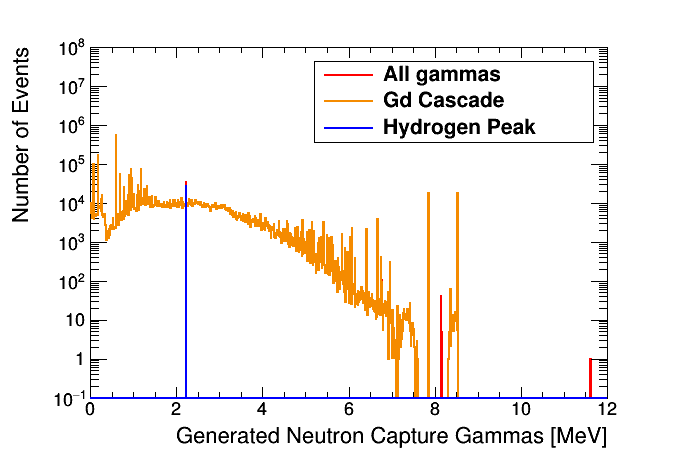
\includegraphics[width=0.7\linewidth]{Chapter4/Figs/Raster/gadolinium/gdCascadeVsAllGammas.png}
 \captionof{figure}{blah.} %~can be used as a kind of place holder in latex
 \label{fig:gdCascadeVsAllGammas}
\end{figure}

\begin{figure}[htbp]
 \centering
 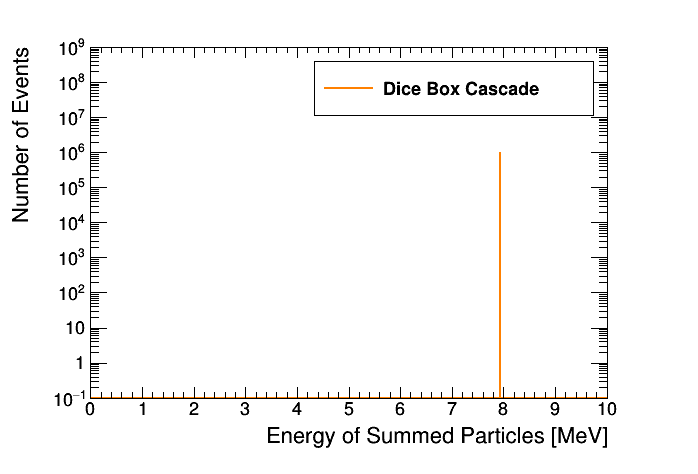
\includegraphics[width=0.7\linewidth]{Chapter4/Figs/Raster/gadolinium/conservationOfCascadeGd.png}
 \captionof{figure}{blah.} %~can be used as a kind of place holder in latex
 \label{fig:conservationOfCascadeGd}
\end{figure}

\begin{figure}[htbp]
 \centering
 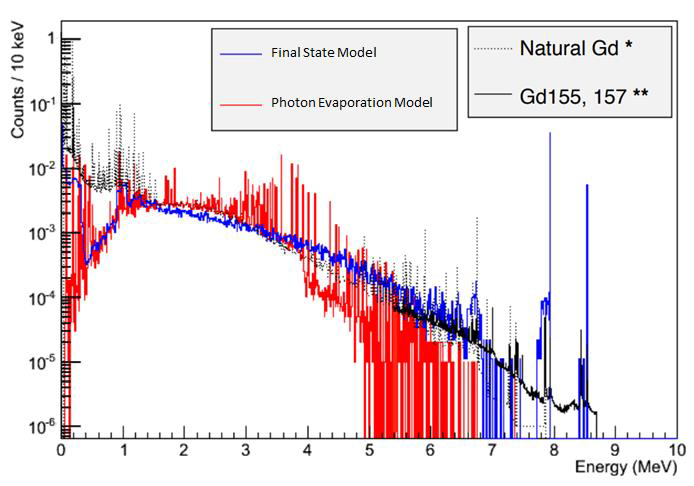
\includegraphics[width=0.7\linewidth]{Chapter4/Figs/Raster/gadolinium/comparisonGd.png}
 \captionof{figure}{blah. * \cite{kandlakunta_2012} ** \cite{bollinger_1970} from \cite{YuChen_2015}} %~can be used as a kind of place holder in latex
 \label{fig:comparisonGd}
\end{figure}

\begin{figure}[htbp]
 \centering
 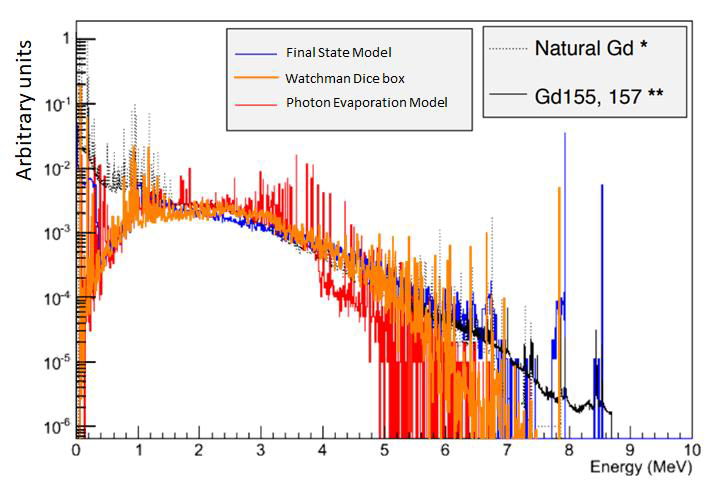
\includegraphics[width=0.7\linewidth]{Chapter4/Figs/Raster/gadolinium/comparisonAndDiceBoxGd.png}
 \captionof{figure}{blah. \ref{fig:energyOfCascadeOfCascadeGd} * \cite{kandlakunta_2012} ** \cite{bollinger_1970} from \cite{YuChen_2015}} %~can be used as a kind of place holder in latex
 \label{fig:comparisonAndDiceBoxGd}
\end{figure}
 
\begin{figure}[htbp]
 \centering
 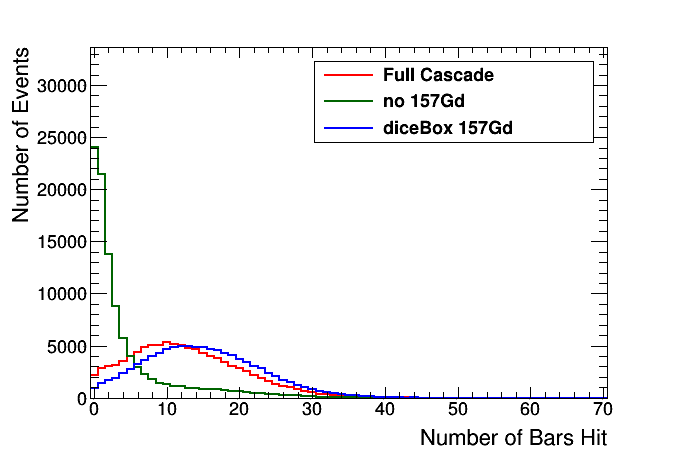
\includegraphics[width=0.7\linewidth]{Chapter4/Figs/Raster/gadolinium/numberOfBarsHitCascadeFinalStateDicebox.png}
 \captionof{figure}{blah.} %~can be used as a kind of place holder in latex
 \label{fig:numberOfBarsHitCascadeFinalStateDicebox}
\end{figure}


\section{Machine Learning Neutron Trigger}\label{sec:MachineLearningTrigger}
Using simulated data is is possible to test weather a machine learning trigger would be advantageous to the analysis. The machine learning technique used was a Support Vector Machine (SVM) \cite{Boser92atraining} \cite{cortes1995support}. SVMs were considered after comparing several other simple techniques that are typically used such as a decision tree and k nearest neighbours the results of this can be seen in figure \ref{fig:sklearnReleventExamples}. As seen in figure \ref{fig:sklearnReleventExamples} the SVM can be used in its pure linear classification form or with a kernel the radial basis function (RBF) kernel is one of the most common. In figure \ref{fig:sklearnReleventExamples} the generalised boundaries, high accuracy, and well defined confidence space seen in the RBF SVM makes it the clear standout. The SVM has used the kernel trick since at least 1992 \cite{Boser92atraining} in figure \ref{fig:svmBoser92LinearSVM} how the support vectors influence the best separating hyper-plane can be seen. SVMs can have different kernels used with them as figure \ref{fig:svmBoser92KernelSVM} shows the results are similar weather a polynomial or RBF kernel is used. Providing the kernel can effectively transform data so that it becomes linearly separable the SVM will be able to separate the data as shown by figure \ref{fig:kernelRBF_fromWeB}. A further test of the RBF SVM's capabilities was done in figure \ref{fig:svmExp_GausseExamples} which tested exponential noise in the x-y plane and two signal Gaussian peaks. As a result it is possible to see that the RBF SVM can draw complicated boundaries around complex signal and noise. 
\\\\A support vector machine is also convexly optimised which means the solutions are easier to solve for as there is only one global minimum \cite{cortes1995support}. The draw backs of SVMs are the long training times relative to other machine learning techniques  due to the maths behind the solution for the SVM being a squared problem to solve\cite{cortes1995support}. This means that for data with many dimensions and many statistics training times and memory usage can be very high to the point of being unusable \cite{cortes1995support}. Data must also be completely labelled and optimisation for training whilst possible through sequential minimal optimisation is somewhat limited \cite{platt1998sequential}. These drawbacks are not a significant issue for the trigger data but they should be bared in mind for more complex cases such as image recognition.
 
\begin{figure}[htbp]
\centering
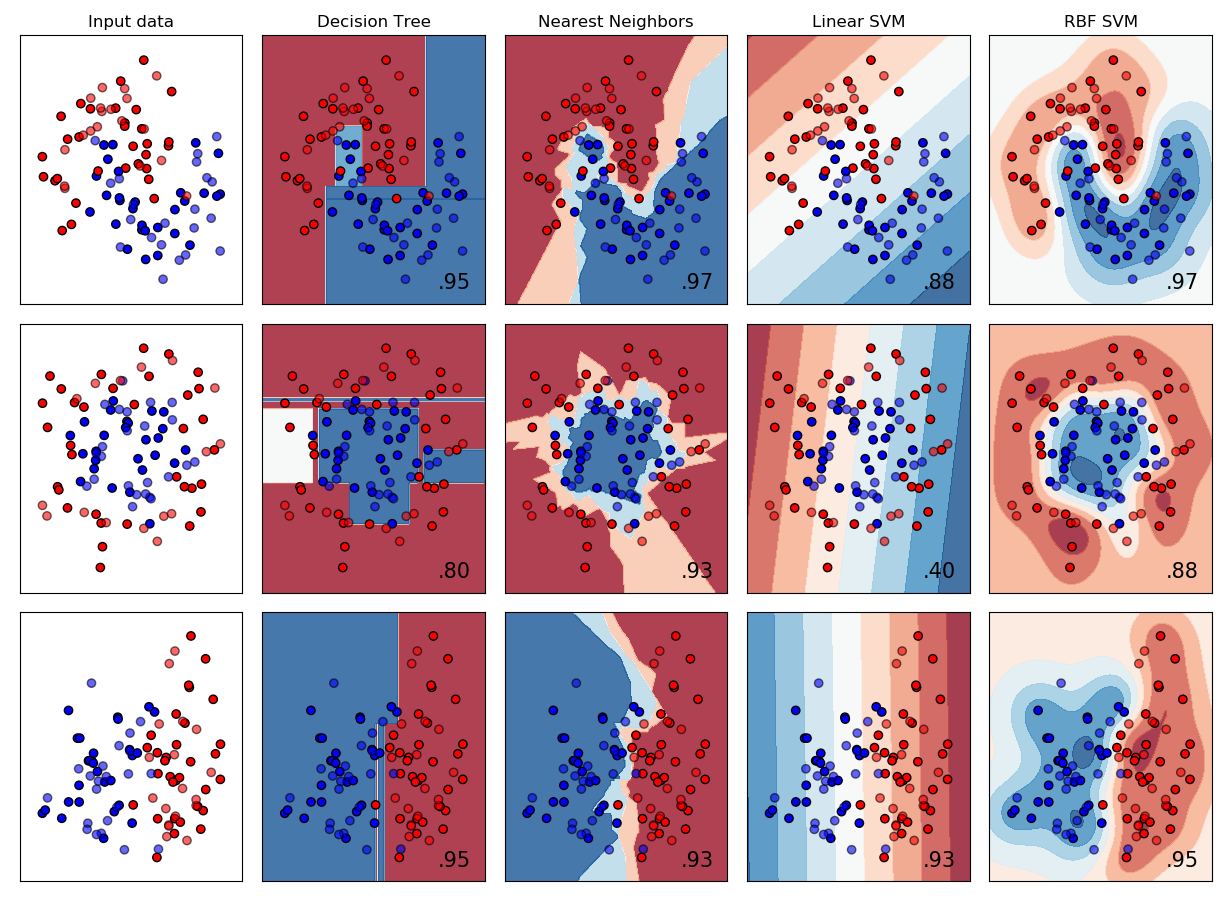
\includegraphics[width=\linewidth]{Chapter4/Figs/Raster/svmLinAndRbf/sklearnReleventExamples.png}
\captionof{figure}{Some example classifiers taken from scikit-learn that show how different techniques draw boundaries and how confident they are in those boundaries. Decision trees and k nearest neighbours are common simplistic classifiers used in physics but the boundaries they produce are often susceptible to over-training. The linear SVM is generalised but is quite limited in its utility. The SVM with the RBF kernel consistently draws the most accurate boundaries and they are well generalised. The accuracy of each technique is shown in the bottom right of each plot from \cite{scikit-learn}.} 
\label{fig:sklearnReleventExamples}
\end{figure}

\begin{figure}[htbp]
\centering
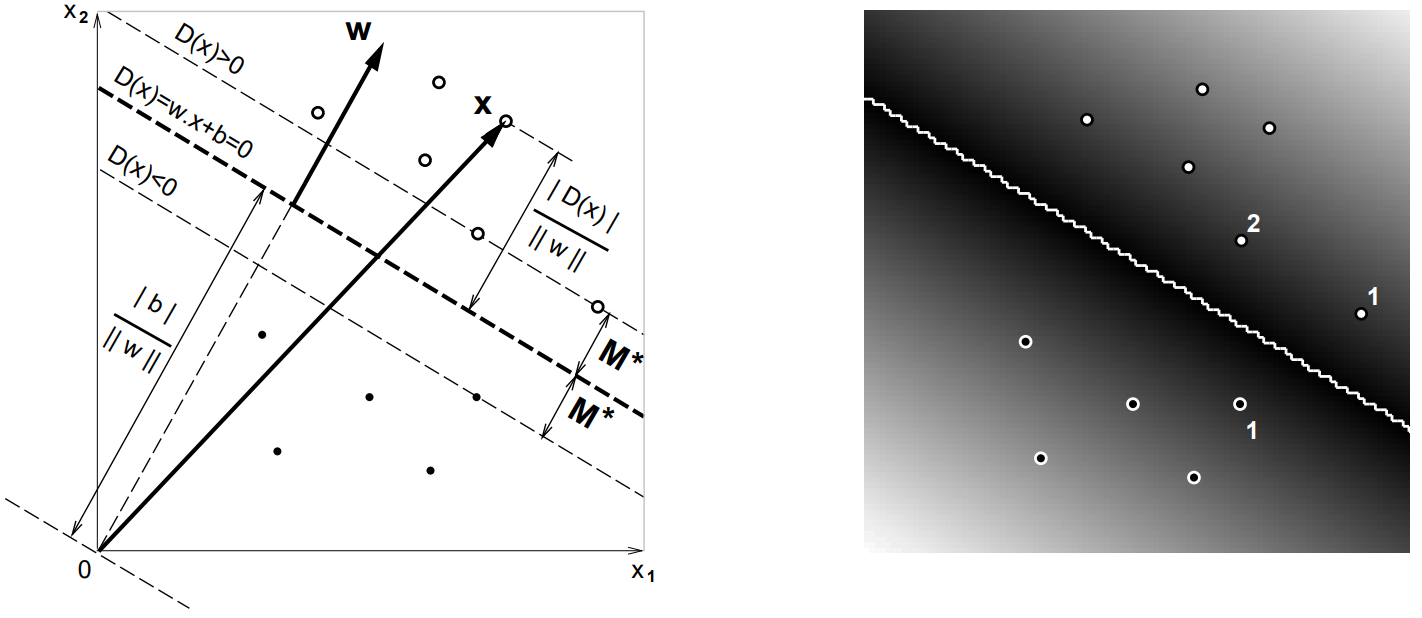
\includegraphics[width=\linewidth]{Chapter4/Figs/Raster/svmLinAndRbf/svmBoser92LinearSVM.png}
\captionof{figure}{An example of a how a support vector machine (SVM) separates two different distributions that are linearly separable. The maths behind the classifier finds the best separating line/hyper-plane between two distributions from \cite{Boser92atraining}.} 
\label{fig:svmBoser92LinearSVM}
\end{figure}

\begin{figure}[htbp]
\centering
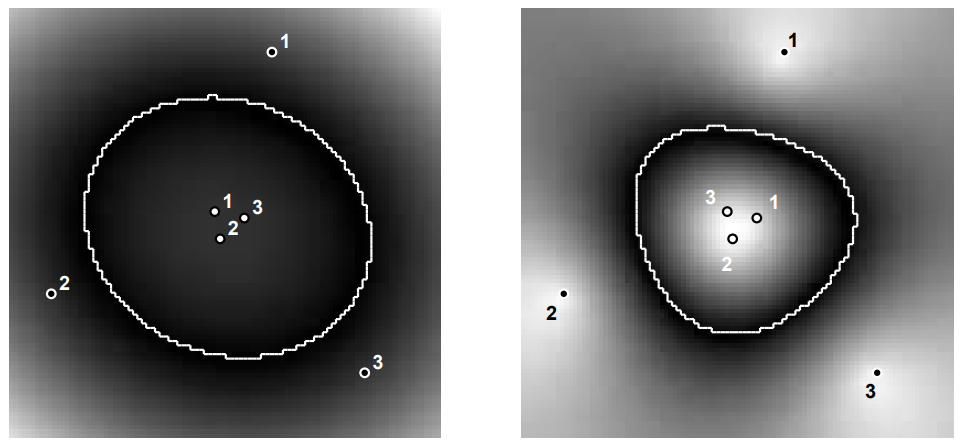
\includegraphics[width=\linewidth]{Chapter4/Figs/Raster/svmLinAndRbf/svmBoser92KernelSVM.png}
\captionof{figure}{How a support vector machine (SVM) operates with a kernel being applied using a squared polynomial kernel on the left and a radial basis function (RBF) on the right . By using the ``kernel trick'' it is now possible to separate non-linear data from \cite{Boser92atraining}.} 
\label{fig:svmBoser92KernelSVM}
\end{figure}

\begin{figure}[htbp]
\centering
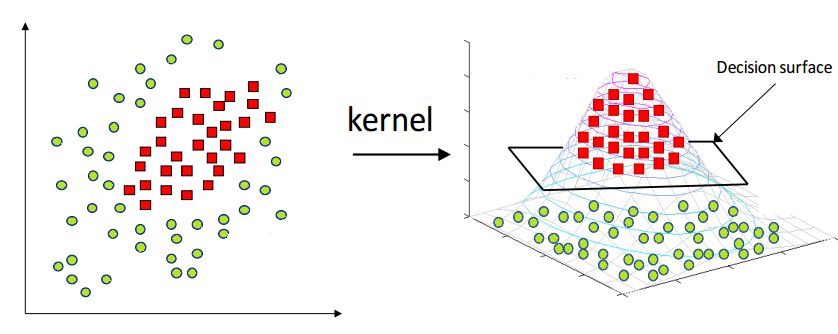
\includegraphics[width=\linewidth]{Chapter4/Figs/Raster/svmLinAndRbf/kernelRBF_fromWeB.png}
\captionof{figure}{An online example that shows how the kernel trick is used to make non-linear data linearly separable by transforming it through a kernel. From \url{https://medium.com/@zxr.nju/what-is-the-kernel-trick-why-is-it-important-98a98db0961d}.} 
\label{fig:kernelRBF_fromWeB}
\end{figure}

\begin{figure}[htbp]
\centering
\begin{subfigure}{.5\textwidth}
  \centering
  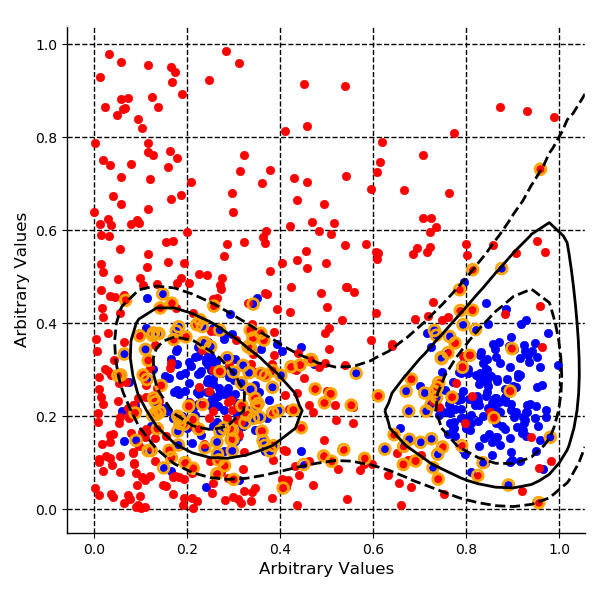
\includegraphics[width=\linewidth]{Chapter4/Figs/Raster/svmLinAndRbf/svmExp_2GaussExample.png}
  \captionsetup{width=.9\linewidth}
  \caption{How LIBSVM draws boundaries around complex signal and noise data sets with an RBF kernel. Support vectors highlighted in orange.}
  \label{subFig:svmExp_2GausseExample}
\end{subfigure}%
\begin{subfigure}{.5\textwidth}
  \centering
  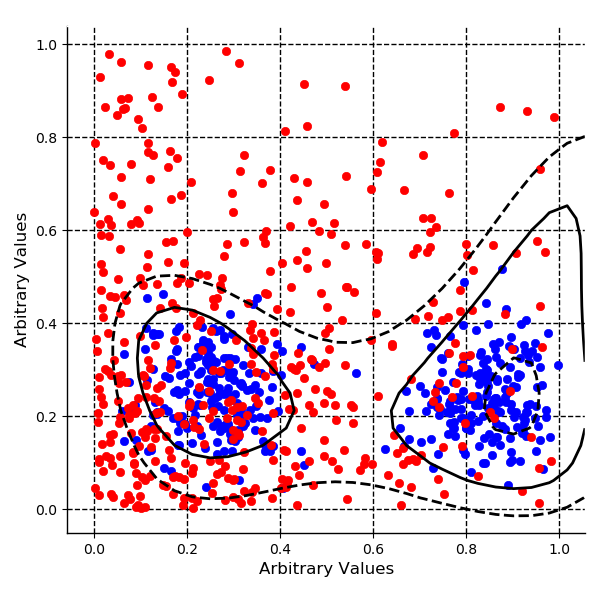
\includegraphics[width=\linewidth]{Chapter4/Figs/Raster/svmLinAndRbf/exp_2NysGaussExample.png}
  \captionsetup{width=.9\linewidth}
  \caption{How LIBLINEAR draws boundaries around complex signal and noise sets with a Nystrom approximation of the RBF kernel with a sampling of 100.}
  \label{subFig:exp_2NysGaussExample}
\end{subfigure}
\caption{SVM examples showing how to separate data sets with two Gaussian signals (blue) from exponential noise (red). For both an RBF kernel was used with c = 1e4 and $\gamma$ = 1.}
\label{fig:svmExp_GausseExamples}
\end{figure}

Figures \ref{fig:sklearnReleventExamples} \ref{fig:svmBoser92LinearSVM} \ref{fig:svmBoser92KernelSVM} \ref{fig:kernelRBF_fromWeB} \ref{fig:svmExp_GausseExamples} are sufficient reason to believe that an SVM with an RBF kernel should be a suitable classifier for separating trigger data which only has four dimensions. The four dimensions that need to be optimised are: the summed energy above a threshold of 1.5\,PE (0.06\,MeV), summed energy above a threshold of 12.5\,PE (0.5\,MeV), Numbers of bars hit above a threshold of 1.5\,PE (0.06\,MeV), Numbers of bars hit above threshold 12.5\,PE (0.5\,MeV). The libraries used were LIBSVM and LIBLINEAR both of which are highly provident and are often cited as reason for the SVMs gain in popularity \cite{chang2011libsvm} \cite{fan2008liblinear} \cite{murty2016support}. The wrapper in sci-kit learn was the preferred method due to its ease of use and its convenient application of the Nystrom approximation \cite{williams2001using} of the kernel. The Nystroem approximation is useful as the amount of computation required for complete kernel SVMs scales $\sim$ O (n$^3$) where n is the number of training examples \cite{williams2001using}. By using a sample of size m to compute an approximation of the kernel the amount of computation required scales $\sim$ O (m$^2$n) instead \cite{williams2001using}. This approach will work even when m $\ll$ n \cite{williams2001using}. The example data shown in \ref{fig:svmExp_GausseExamples} shows how LIBLINEAR when combined with with an RBF Nystroem approximated kernel performs in comparison to LIBSVM with a complete RBF kernel the boundaries are very similar. From this point the LIBLINEAR library and the Nystroem approximation will be used to speed up training and to prevent memory overflow which can happen when the SVM isn't converging and when large data sets are used. 
\\\\Kernel SVMs have two factors that can be tweaked to give more accurate results. The soft margin C where high values minimise error as much as possible and low values try to generalise as much possible which approach is best will depend on the data set being analysed \cite{cortes1995support}. Typically C can vary from 10$^-6$ to 10$^6$ but can be even higher or even lower. The other factor is $\gamma$ and is part of the RBF kernel shown in equation \ref{equ:RbfKernelFunc} and is taken from \cite{Boser92atraining}. The value for $\gamma$ must be $>$ 0. For an example of what non linear data looks like when searching for suitable C and $\gamma$ values figure \ref{fig:GammaCGridSearchExp2Gauss} was produced which shows how the values for figure \ref{subFig:exp_2NysGaussExample} where chosen. A higher value of $\gamma$ corresponds to higher non-linearity and a higher value of C corresponds to a lower overlap. With this information we can see that there is some overlap in figure \ref{subFig:exp_2NysGaussExample} and is very non linear so this search for relevant C and $\gamma$ values corroborates what can be seen in the example data. In contrast the generated neutron and noise data shows clear linearity as low $\gamma$ values are preferred and has small overlap as high C values are preferred. This shows that the generated neutron data is very easy to separate with a linear classifier and so using anything more than a support vector machine would be unlikely to yield better results.

\begin{equation}
K(\mathbf{x,x'}) = \exp{(\gamma \mathbf{x \cdot x'})} - 1
\label{equ:RbfKernelFunc}
\end{equation}

\begin{figure}[htbp]
\centering
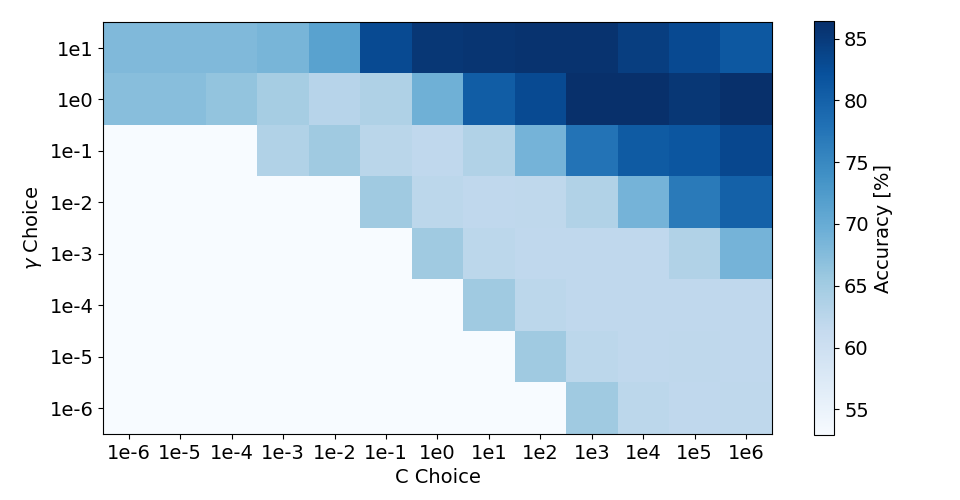
\includegraphics[width=0.9\linewidth]{Chapter4/Figs/Raster/GammaCGridSearchExp2Gauss.png}
\captionof{figure}{SVMs being trained on varying values of C and $\gamma$ for figure \ref{subFig:exp_2NysGaussExample}. Higher values of $\gamma$ represent non-linear data separation which the SVMs settle on. Higher values of C represent more overlap in the data. This is less clear but ultimately a higher value of C was settled due to a high preference for isolating boundaries as much as possible. A $\gamma$ = 1e0 and C of 1e4 was chosen.} %~can be used as a kind of place holder in latex
\label{fig:GammaCGridSearchExp2Gauss}
\end{figure}

\begin{figure}[htbp]
\centering
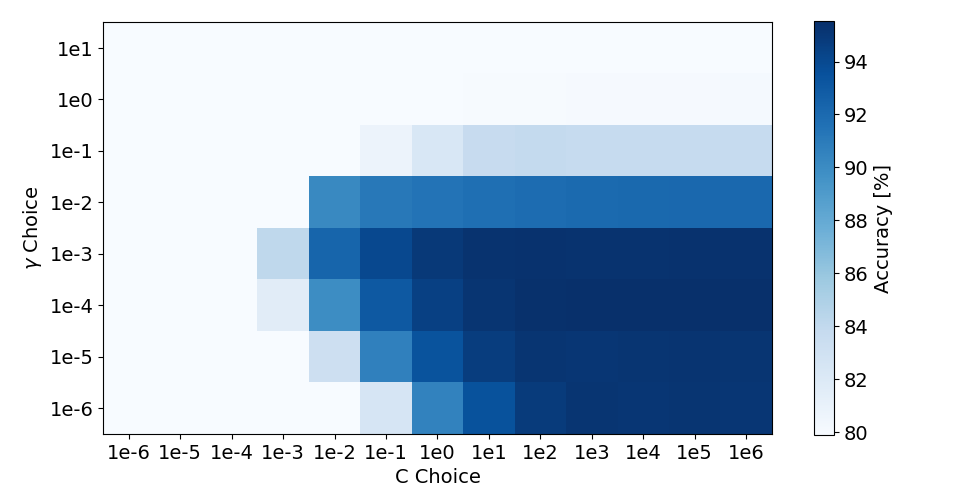
\includegraphics[width=0.9\linewidth]{Chapter4/Figs/Raster/GammaCGridSearchNeutron.png}
\captionof{figure}{SVMs being trained on varying values of C and $\gamma$ for figure generated noise and neutron data. Lower values of $\gamma$ represent a linear data separation which the SVMs settle on. Higher values of C represent more overlap in the data. This data set is linearly separable with minimal overlap. A $\gamma$ = 1e-6 and C of 1e6 was chosen.} %~can be used as a kind of place holder in latex
\label{fig:GammaCGridSearchNeutron}
\end{figure}

In addition it is then possible to perform a basic form of dimensional reduction by seeing how the various dimensions effect the accuracy of the classifier which can be seen in figure \ref{fig:accNeutronSVMC1e6_g1e-6}. In figure \ref{fig:accNeutronSVMC1e6_g1e-6} the addition of more dimensions beyond 2 dimensions does not seem to increase accuracy suggesting that not all of the information provided by the emulated trigger is useful. This is also true for efficiency as seen in figure \ref{fig:effNeutronSVMC1e6_g1e-6} and purity as seen in figure \ref{fig:purNeutronSVMC1e6_g1e-6}. The most accurate would be the summed energy above a threshold of 1.5\,PE and the number of bars hit above 1.5\,PE. However, the easier to implement option would be to use the number of bars hit above 1.5\,PE and the number of bars hit above 12.5\,PE for the electronics on VIDARR. As the drop in accuracy efficiency and purity was relatively low for this combination this was the preferred option. The result of which can be seen in figure \ref{fig:signalAndNoiseNeutronSVM_C1e6_g1e-6}.

\begin{figure}[htbp]
\centering
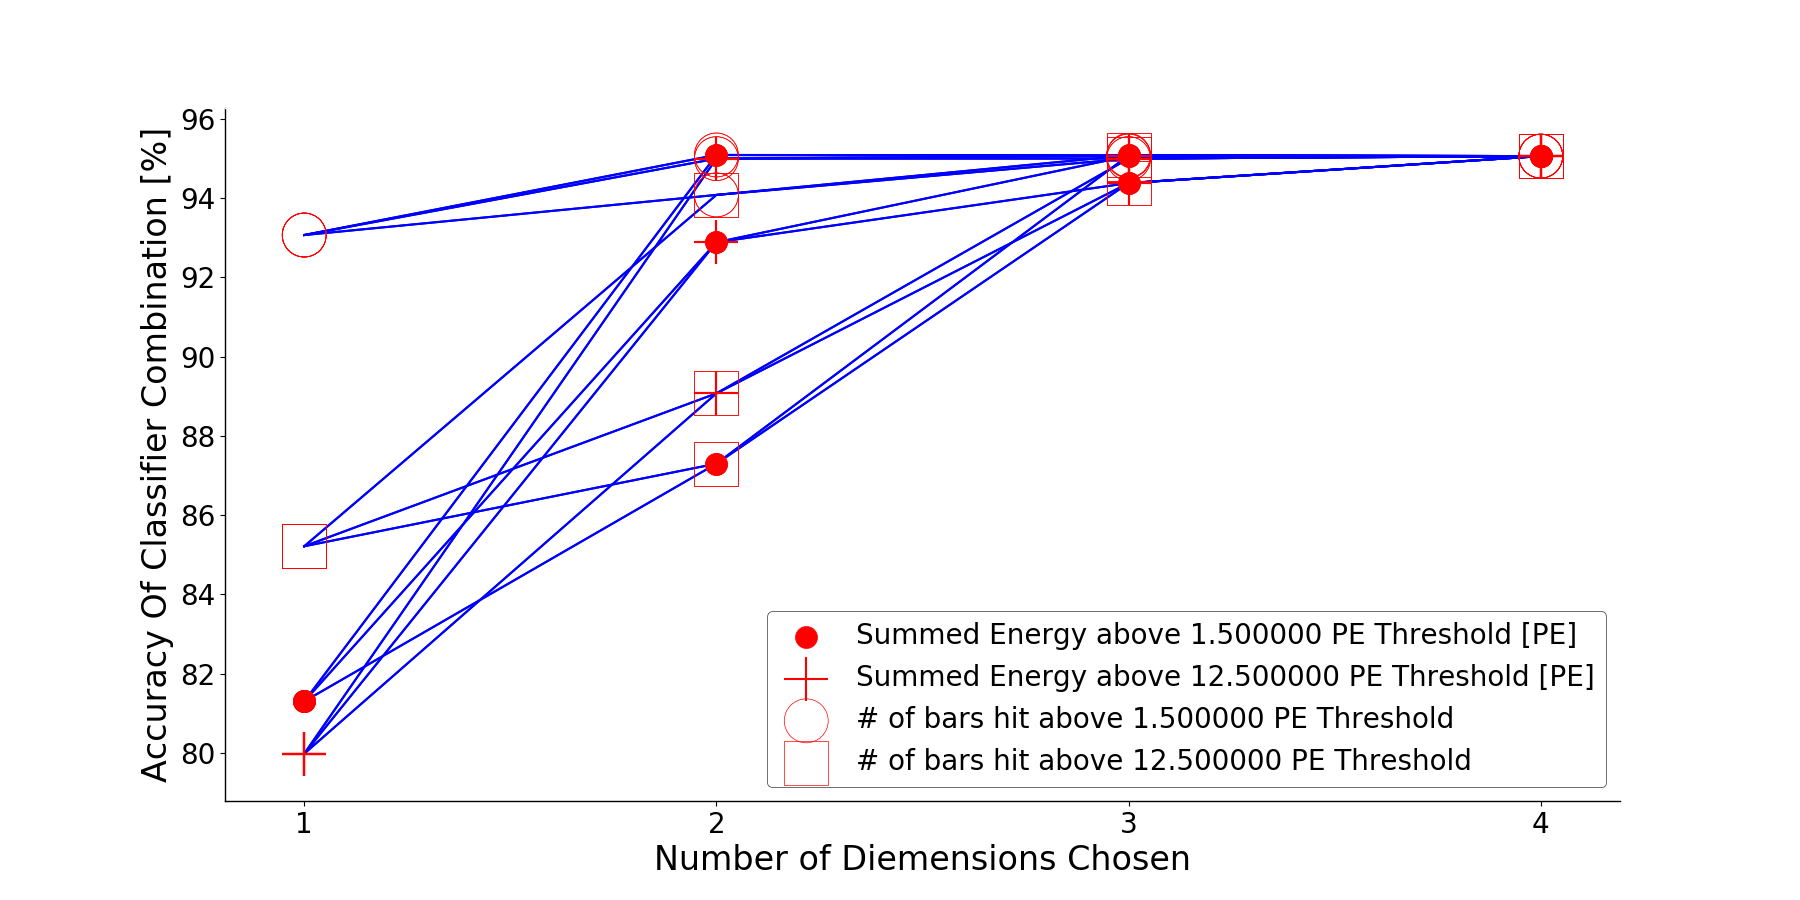
\includegraphics[width=\linewidth]{Chapter4/Figs/Raster/accNeutronSVMC1e6_g1e-6.png}
\captionof{figure}{The accuracy for Nystroem SVM classifiers with approximate RBF kernel with sample of 100 for generated neutron and noise data. With C = 1e6 and $\gamma$ = 1e-6. Separation don't improve above 2 dimensions.} %~can be used as a kind of place holder in latex
\label{fig:accNeutronSVMC1e6_g1e-6}
\end{figure}

\begin{figure}[htbp]
\centering
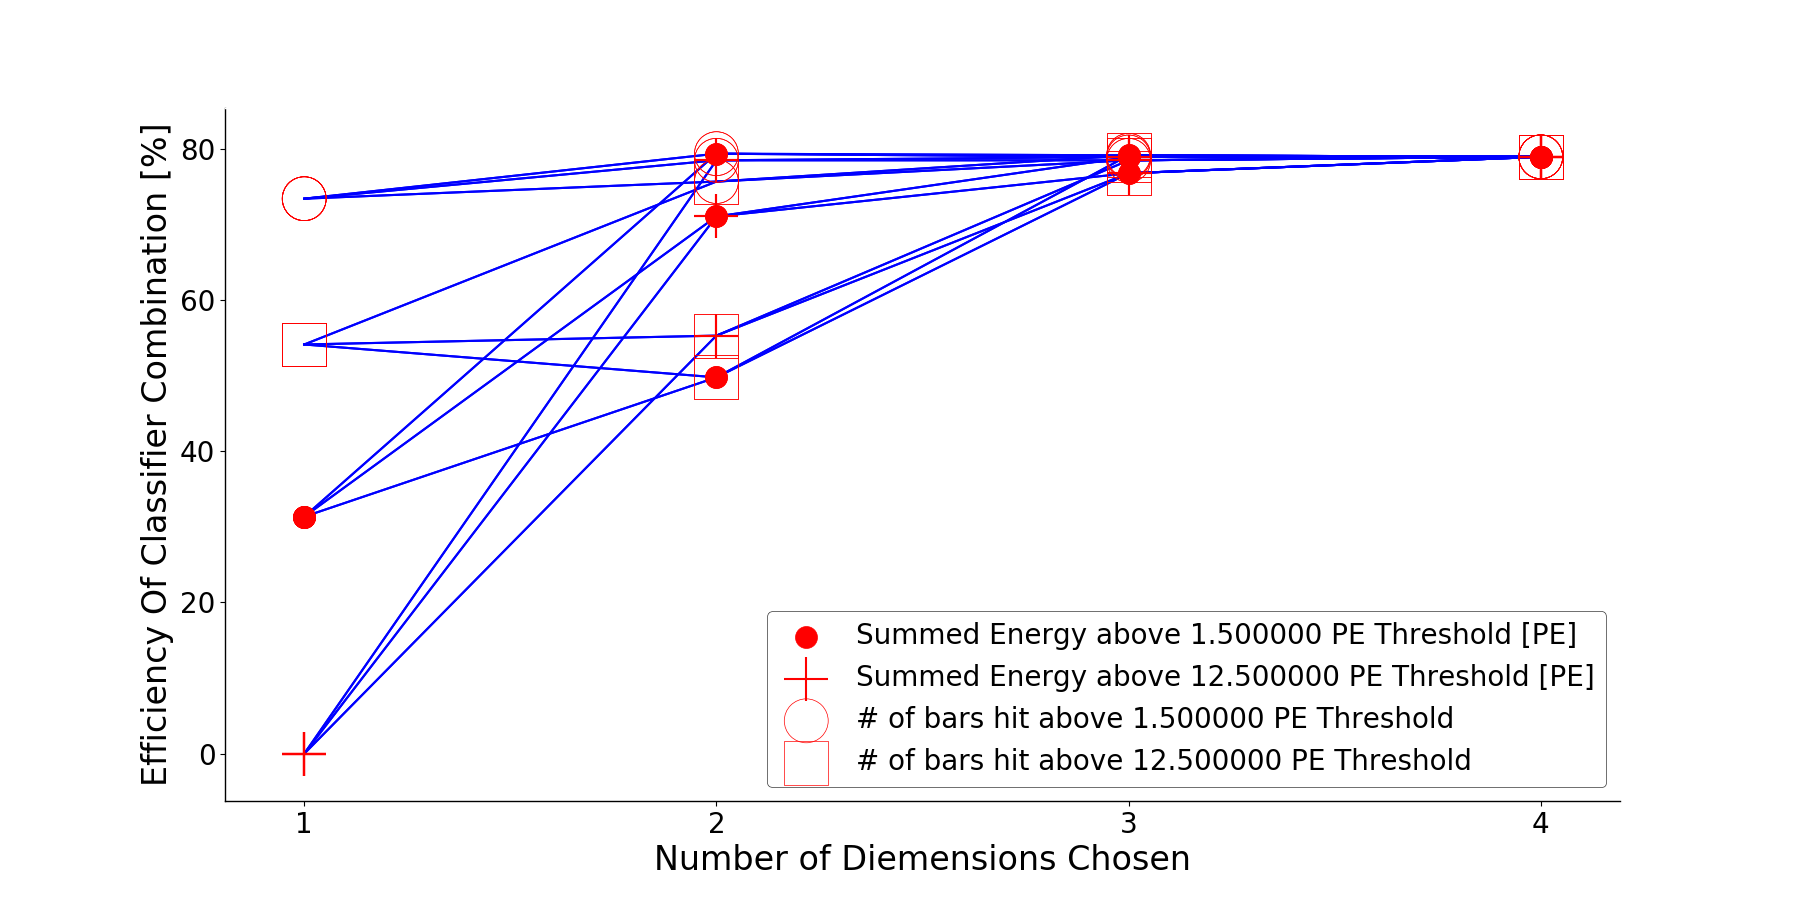
\includegraphics[width=\linewidth]{Chapter4/Figs/Raster/effNeutronSVMC1e6_g1e-6.png}
\captionof{figure}{The efficiency for Nystroem SVM classifiers with approximate RBF kernel with sample of 100 for generated neutron and noise data. With C = 1e6 and $\gamma$ = 1e-6. Separation don't improve above 2 dimensions.} %~can be used as a kind of place holder in latex
\label{fig:effNeutronSVMC1e6_g1e-6}
\end{figure}

\begin{figure}[htbp]
\centering
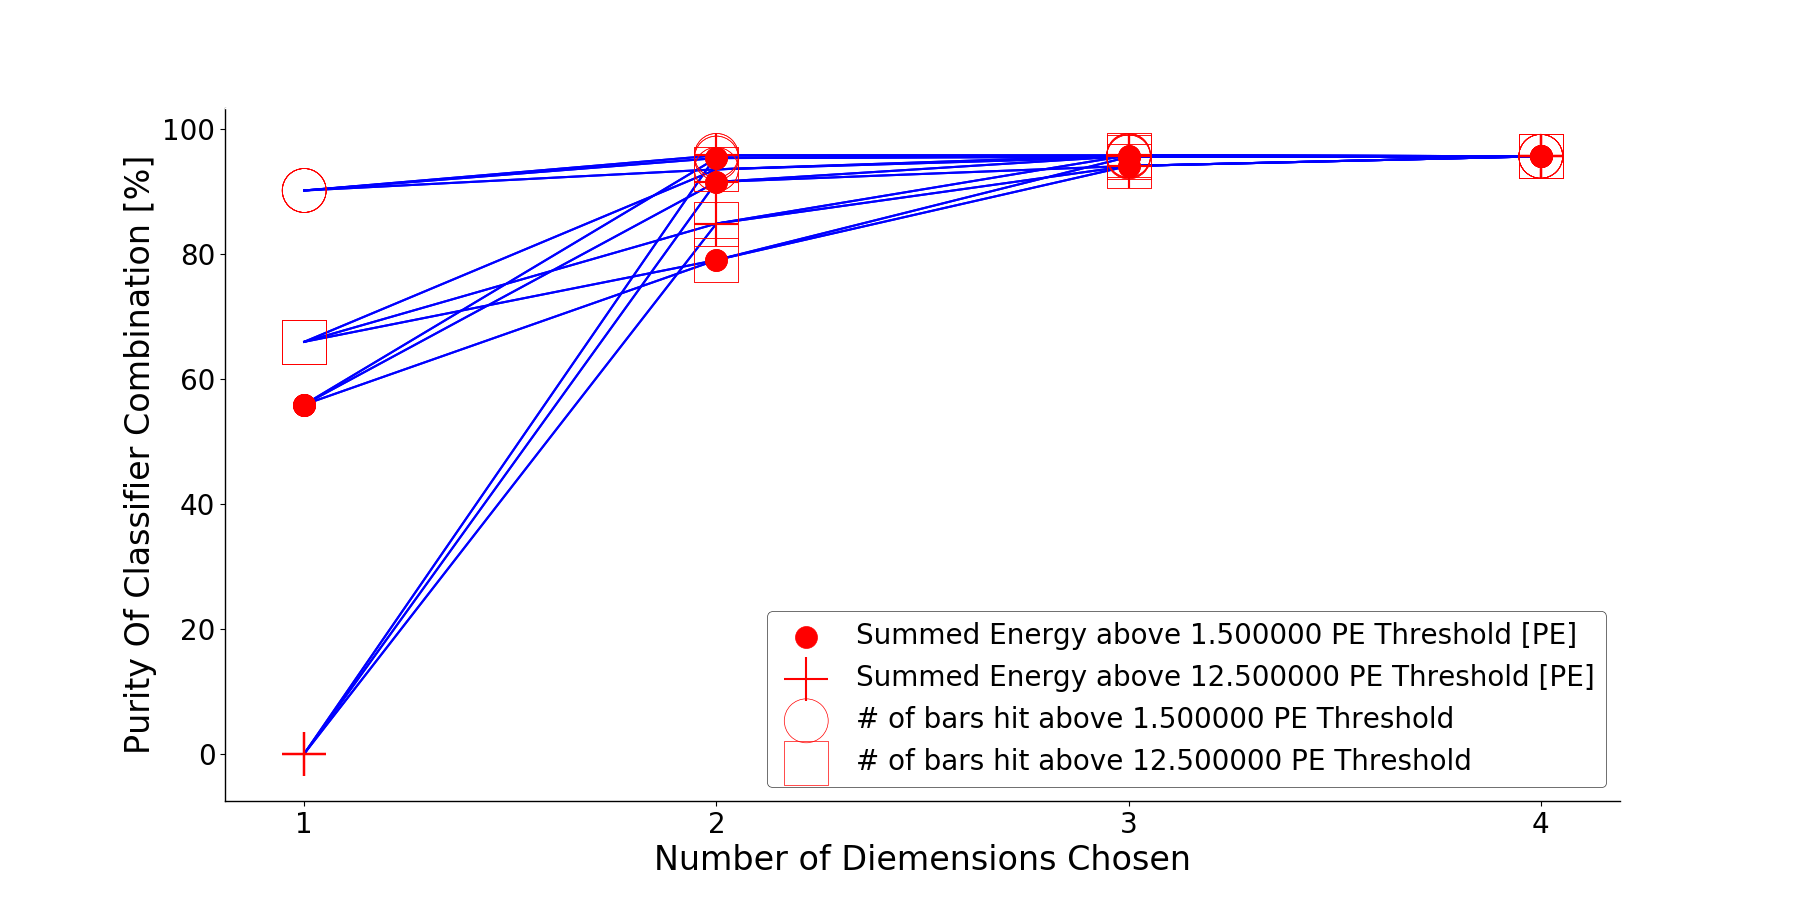
\includegraphics[width=\linewidth]{Chapter4/Figs/Raster/purNeutronSVMC1e6_g1e-6.png}
\captionof{figure}{The purity for Nystroem SVM classifiers with approximate RBF kernel with sample of 100 for generated neutron and noise data. With C = 1e6 and $\gamma$ = 1e-6. Separation don't improve above 2 dimensions.} %~can be used as a kind of place holder in latex
\label{fig:purNeutronSVMC1e6_g1e-6}
\end{figure}

In figure \ref{fig:signalAndNoiseNeutronSVM_C1e6_g1e-6} anything to the left of the line is considered noise event and anything to the right of the line is considered a neutron event. The effect of this selection criteria can be seen in figure \ref{fig:summedEnergyPastTriggerGdDicebox} which shows the summed energy that makes it past the emulated trigger. The amount of summed energy past the emulated trigger is overwhelmingly dominated by the 8\,MeV $\gamma$ cascade from neutron absorption. The only events that are able to make it past the emulated trigger are the electrons with initial high kinetic energies as seen in figure \ref{fig:GeneratedEnergyPastTriggerGdDicebox} but they are unlikely to be present when in sufficient quantities when the detector is deployed. 

\begin{figure}[htbp]
\centering
\begin{subfigure}{.5\textwidth}
  \centering
  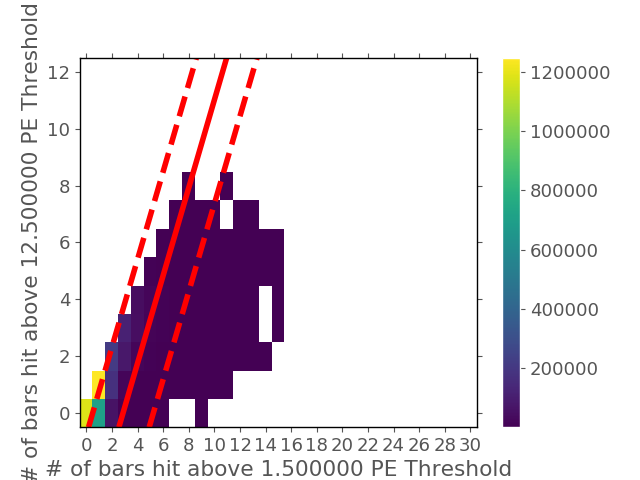
\includegraphics[width=\linewidth]{Chapter4/Figs/Raster/noiseNeutronSVM_C1e6_g1e-6.png}
  \captionsetup{width=.9\linewidth}
  \caption{Generated noise data mainly concentrated at a small number of bar hits.}
  \label{subFig:noiseNeutronSVM_C1e6_g1e-6}
\end{subfigure}%
\begin{subfigure}{.5\textwidth}
  \centering
  \includegraphics[width=\linewidth]{Chapter4/Figs/Raster/signalNeutronSVM_C1e6_g1e-6.png}
  \captionsetup{width=.9\linewidth}
  \caption{Generated neutron $\gamma$ cascade signal which hits many bars.}
  \label{subFig:signalNeutronSVM_C1e6_g1e-6}
\end{subfigure}
\caption{A 2d SVM classifier trained on signal and noise data with number of bars hit above 1.5\,PE (0.06\,MeV) and number of bars hit above 12.5\,PE (0.5\,MeV) with a Nystrom approximate RBF kernel with sampling of 100, C value of 1e6 and $\gamma$ value of 1e-6.}
\label{fig:signalAndNoiseNeutronSVM_C1e6_g1e-6}
\end{figure}

\begin{figure}[htbp]
 \centering
 \includegraphics[width=0.7\linewidth]{Chapter4/Figs/Raster/gadolinium/summedEnergyPastTriggerGdDicebox.png}
 \captionof{figure}{The summed energy past the simulated neutron trigger shown in figure \ref{fig:signalAndNoiseNeutronSVM_C1e6_g1e-6}. 25\,PE = 1\,MeV overall giving an Efficiency = 75.6\,\% and purity = 93.5\,\%. Purity is determined from noise of 4 million noise evetns and 1 million signal events.} %~can be used as a kind of place holder in latex
 \label{fig:summedEnergyPastTriggerGdDicebox}
\end{figure}

\begin{figure}[htbp]
 \centering
 \includegraphics[width=0.7\linewidth]{Chapter4/Figs/Raster/gadolinium/GeneratedEnergyPastTriggerGdDicebox.png}
 \captionof{figure}{The generated kinetic energy for particles which make it past the simulated neutron trigger. The only particles of concern are electrons that produce high enough energy to hit many bars and produce showers. Background electrons with energies > 5\,MeV are unlikely to be prevalent during deployment.} %~can be used as a kind of place holder in latex
 \label{fig:GeneratedEnergyPastTriggerGdDicebox}
\end{figure}

%*******************************************************************************
%***************************************  End  *********************************
%*******************************************************************************